\documentclass[11pt, a4paper]{article}

% --- Geometry (Fixes the margins) ---
\usepackage[margin=1in]{geometry}

% --- Essential Packages ---
\usepackage[utf8]{inputenc} % Allows international characters
\usepackage{amsmath, amssymb} % Must-haves for math notes
\usepackage{graphicx} % For embedding images
\usepackage{hyperref} % Adds clickable links and a PDF outline
\usepackage[table]{xcolor}
\usepackage{multirow}
\usepackage{booktabs}
\providecommand{\m}{\mathcal{M}}

\usepackage{biblatex}
\addbibresource{bibtex.bib}


\title{\textbf{Ruben New Potentials Notes}}
\author{Sandra Tomàs}
\date{June 2026}

\begin{document}

\maketitle

\begin{abstract}
    As now we have lattice data for the potentials $\Sigma_g^+$, $\Pi_u$ and $\Sigma_u^-$ we can change them in the calculation program and recompute the spectrum and also the mixing and the hyperfine splitting.
\end{abstract}


\section{Static Potentials}
For all three potentials we are going to do an interpolation between their behaviour at short- and at long-distances.
\subsection{Short distances}
For short distances we can use perturbative theory from pNRQCD. From \cite{Pineda:2013lta}, we get the perturbative $V^{(0)}$ up to ${\cal O}(\alpha_s^4)$ including the leading ultrasoft corrections $\delta a_3^{us}[\nu,\nu_{us}]$, and the leading renormalon ambiguity ($C_f=(N_c^2-1)/(2N_c)$, $C_A=N_c$)
\begin{align}
    V^{(0)}=&
-\frac{C_f \ \alpha_s}{r}\left[1+
\sum_{n=1}^{3} 
\left(\frac{\alpha_s}{4\pi}\right)^n a_{n}(\nu,\nu_{us} ; r)\right]+2 \delta m_{RS'}(\nu_f) \, ,
\end{align}
up to this order the coefficients $a_n$ are completely known:
\begin{eqnarray}
a_1(\nu;r)
&=&
a_1+2\beta_0\,\ln\left(\nu e^{\gamma_E} r\right)
\,,
\nonumber\\
a_2(\nu;r)
&=&
a_2 + \frac{\pi^2}{3}\beta_0^{\,2}
+\left(\,4a_1\beta_0+2\beta_1 \right)\,\ln\left(\nu e^{\gamma_E} r\right)\,
+4\beta_0^{\,2}\,\ln^2\left(\nu e^{\gamma_E} r\right)\,
\,,
\nonumber \\
a_3(\nu;r)
&=&
a_3+ a_1\beta_0^{\,2} \pi^2+
\frac{5\pi^2}{6}\beta_0\beta_1 +{\color{red}16}\zeta_3\beta_0^{\,3}
\nonumber \\
&+&\bigg(2\pi^2\beta_0^{\,3} 
+ 6a_2\beta_0+4a_1\beta_1+2\beta_2
+\frac{16}{3}C_A^{\,3}\pi^2\bigg)\,
  \ln\left(\nu e^{\gamma_E} r\right)\,
\nonumber \\
&+&\bigg(12a_1\beta_0^{\,2}+10\beta_0\beta_1\bigg)\,
  \ln^2\left(\nu e^{\gamma_E} r\right)\,
+8\beta_0^{\,3}  \ln^3\left(\nu e^{\gamma_E} r\right)\,
\nonumber
\\
&+&\delta a_3^{us}(\nu,\nu_{us}).
\label{eq:Vr}
\end{eqnarray}
{\color{red} The factor $16$ is $13$ in Ruben's code and mine, should be checked.}
For the
ultrasoft corrections to the static potential we take
\begin{equation}
\delta a_3^{us}(\nu,\nu_{us})
%={8 C_A^3\over
%  3\beta_0}\pi^2 \ln\left(
%\alpha_{s}(\nu)\over \alpha_{s}(\nu_{us}) \right)
= \frac{16}{3}C_A^3 \pi^2\ln\left(\frac{\nu_{us}}{\nu}\right)
\, .
\end{equation}
The $\delta m_{RS'}(\nu_f)$ term appears to correct the shifting due to renormalons and can be expressed as a series in different orders in perturbation theory. It depends on $0$, $1$, or $2$ loop terms around the renormalon and it reads as
\begin{equation}
    \delta m_{RS'}(\nu,\nu_f) = \nu_f \Big[ \alpha_S
(\nu) \delta m^{(0)} + \alpha_S^2
(\nu) \delta m^{(1)} + \alpha_S^3
(\nu) \delta m^{(2)} + \alpha_S^4
(\nu) \delta m^{(3)} \Big]
\end{equation}
Having from \cite{Pineda:2013lta} $\delta m^{(0)}=0$ and 
$d_n(\nu,\nu_f)=\beta_n/2^{1+2n}\ln\left(\frac{\nu}{\nu_f}\right)$
\begin{equation}
\begin{split}
&
\delta m^{(1)}(\frac{\nu_f}{\nu})= N_m
\frac{\beta_{0}}{2\pi} S(1,b), \\
&
\delta m^{(2)}(\frac{\nu_f}{\nu})= N_m\left(\frac{\beta_{0}}{2\pi}\right)
\left[ S(1,b)
\frac{2d_{0}(\nu,\nu_{f})}{\pi} + \left(\frac{\beta_{0}}{2\pi}\right) S(2,b)
\right], \\
&
\begin{split}
\delta m^{(3)}(\frac{\nu_f}{\nu}) =& N_m \left(\frac{\beta_{0}}{2\pi}\right)\times \\
&
\times \left[ 
S(1,b) \frac{3d_{0}^{2}(\nu,\nu_{f})+2d_{1}(\nu,\nu_{f})}{\pi^{2}} +
\left(\frac{\beta_{0}}{2\pi}\right) S(2,b) \frac{3d_{0}(\nu,\nu_{f})}{\pi} +
\left(\frac{\beta_{0}}{2\pi}\right)^{2} S(3,b) \right].
\end{split}
\end{split}
\end{equation}
where
\begin{equation}
S(n,b)=\sum_{k=0}^2c_k\frac{\Gamma(n+1+b-k)}{\Gamma(1+b-k)}
\end{equation}
with $c_0=1$ and 
\begin{equation}
b={\beta_1 \over 2\beta_0^2}\,,
\qquad
c_1={1 \over 4\,b\beta_0^3}\left({\beta_1^2 \over \beta_0}-\beta_2\right)
\end{equation}
and 
\begin{equation}
c_2={1 \over b(b-1)}
{\beta_1^4 + 4 \beta_0^3 \beta_1 \beta_2 - 2 \beta_0 \beta_1^2 \beta_2 + 
   \beta_0^2 (-2 \beta_1^3 + \beta_2^2) - 2 \beta_0^4 \beta_3 
\over 32 \beta_0^8}
\,.
\end{equation}



With this our \textbf{perturbative} potentials read
\begin{equation}
 V^{\Sigma_g}_{\rm Pert}=V^{(0)},
\qquad \qquad
V^{\Pi_u}_{\rm Pert}=V^{\Sigma_u^-}_{\rm Pert}=-V^{(0)}/8 \, .
\end{equation}
We can see that $V^{\Sigma_g}_{\rm Pert}$ is directly the singlet potential, the other two are the octet perturbative potentials so to write as the singlet we need to scale it using the colour factor $(C_A/2 - C_F)/(-C_F) = -1/8$.
Comparing from short distance lattice data from ref.~\cite{Schlosser:2025tca} we see that to reproduce correctly the data we need to add a global shift. So the \textbf{short distance} potentials finally become
\begin{equation}
    V^{\Lambda_\eta^\sigma}_{\rm Short} = V^{\Lambda_\eta^\sigma}_{\rm Pert} + \mu^{\Lambda_\eta^\sigma}_s \, .
\end{equation}

\subsection{Long distances}
For the long distance we use the expression of EST with the hole contributions. 
\begin{equation}
    V_{\rm EST}(N)=\sqrt{\sigma^2 r^2+2\pi\left(N-\frac{1}{12}\right) \sigma}
\end{equation}
where $\sigma=0.21GeV^2$ is the string tension. $N$ is the excitation levels of the EST potentials \cite{Luscher:2002qv}. For the ground state ($N=0, \Sigma_g$) and the excited strings ($N=1, \Pi_u$ and $N=3, \Sigma_u^-$). We use the expansions truncated up to ${\cal O}(1/r^3)$ for $N=0$, while for the excited states using the full expression shows better convergence.

Once again to fit the lattice data we add a shift this time
\begin{equation}
    V_{\rm Long}^{\Lambda_\eta^\sigma} = V_{\rm EST}^{\Lambda_\eta^\sigma} + \mu_l^{\Lambda_\eta^\sigma} \, .
\end{equation}

\subsection{Interpolation}
The interpolation is done in a very complicated form and the coefficients are exactly adjusted to fit the lattice data the most accurately.
\begin{align}
    V^{\Lambda_\eta^\sigma}_\text{Fit}(r)\quad=\quad\frac{V_\text{Short}(r)\quad+\quad \Lambda_\text{lat}\sum^{k_a}_{j=m} a_j( r/r_c)^j\quad +\quad (r/r_c)^n  \ \  V_\text{Long}(r) }{1\quad \quad +\quad  \sum^{k_b}_{j=m} b_j ( r/r_c)^j\quad+\quad\quad ( r/r_c)^n  \ \ } \, ,
\end{align}
the fitted data being: $n=9$, $m=3$, $k_a=5$, $k_b=4$; and $r_c$, $\mu_s-\mu_l$, $a_j$, $b_j$ which depend on the potential $\Lambda_\eta^\sigma$ in Fig.~\ref{fig:static_coeff}.

\begin{figure}[]
    \centering
    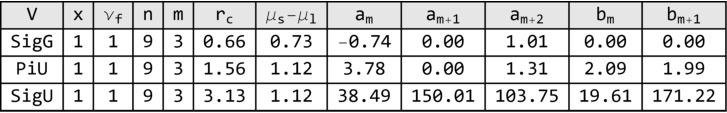
\includegraphics[width=0.6\linewidth]{Fig/coef_hy.pdf}
    \caption{\small Fitting coefficients with first correction $m=3$, last correction $k_a=5$ ($k_b=4$ for the denominator), and spacing $n=9$. We extract $\mu_s-\mu_l$ by adjusting the short and long distance behaviour for short and long Lattice data independently.  }
    \label{fig:static_coeff}
\end{figure}

\section{Static potential matrices}
\begin{itemize}
    \item \textbf{Quarkonium spin 0}: the shape of the potential matrix/hamilonian is 1-dim for every $L=0,1,2$. 
    \begin{equation}
    \label{eq:QS0}
    \frac{\mathcal{J}(\mathcal{J}+1)}{r^2} + m V_{\Sigma_g^+}(r) 
    \end{equation}
%
    \item \textbf{Quarkonium spin 1}: is degenerate with quarkonium spin 0 so the spectrum is the same. This degeneracy is broken by the mixing in next section. Also it could be broken by the hyperfine but in quarkonium this is a NNLO effect.
    \item \textbf{Hybrid spin 0}: the shape of the potential matrices is the one from equations (6) and (7) of \cite{Oncala:2017hop}. In here I flipped the order of the multiplet so our wave function will be
    \[
    \begin{pmatrix}
        P_J^0(r) \\
        P_J^+(r) \\
        P_j^-(r) 
    \end{pmatrix} \, .
    \]
    As $S=0 \to J=\mathcal{J}$. $J=0$ is a special one-dimensional case, for $J \neq 0$ the matrix is three-dimensional. With the mixing we have three more states ordered as in Eq.~\eqref{mat_H04} and \eqref{mat_6x6}.
    \item \textbf{Hybrids spin 1}: as before at the order of the static potentials this spectrum is degenerate with the hybrid spin 0 one. After including the mixing we will break this degeneracy that will be broken further by the inclusion of the hyperfine splitting.
\end{itemize}

\section{Mixing potentials and matrices}
Once undertood this part which is maybe the most tehoretical, the mixing potentials are also given by Ruben with a similar Table. This mixing potentials $V_S^\Sigma$ and $V_S^\Pi$ apear in the mixing matices below. This matrices also contain the regular spectrum potentials, so they are the addition of the last section (regular spectrum) with this one (mixing). All the potentials here are defined by Ruben is his notes.

A very important point here is that in my \texttt{MATLAB} code the implementation of this matrices is done multiplying by $m$ because of the way the coupled-channel Schrödinger equation solving script is constructed. So, everything is multiplied by $m$.

\subsection{Mixing between Quarkonium spin 1 and Hybrid spin 0}
When the hybrid $J=\mathcal{J}$ and the quarkonium $L=\mathcal{J}$
{
\begin{eqnarray}
\label{mat_H04} 
&& 	m_Q\left[ 
 -\frac{1}{m_Q}\frac{\partial^2}{\partial r^2}\!    
	+ \begin{pmatrix}
 		\frac{\mathcal{J}(\mathcal{J}+1)}{m_Q r^2}+\!V_{\Sigma_g^+}  & {\color{red}2V_S^\Pi}                    \\
 		{\color{red}2V_S^\Pi}  & 	\frac{\mathcal{J}(\mathcal{J}+1)}{m_Q r^2}+V_{\Pi_u}                   \\
 	\end{pmatrix}
 	\!
 	-E \right]\! 
	\begin{pmatrix}
 		R_{1\, \mathcal{J}\mathcal{M}}^{0}\\
 		P_{0\, \mathcal{J}\mathcal{M}}^{0} \\
 	\end{pmatrix}\!
 	=0.
\end{eqnarray}
}
{\color{red} $2V_S^\Pi$ is $2V_S^\Sigma$ in Ruben's code. I used $\Pi$ in mine.}
    For $\mathcal{J}= 0$ the equation do not exist: since the gluon spin is 1 for hybrids $(J=L  \oplus 1)$, then only $L=1$ can give $J=0$, which is incompatible with the requirement of the  previous equation $\mathcal{J}=J=L$. \\
    
When the hybrid $J=\mathcal{J}$ and  the quarkonium $L={J \pm 1}$
{ \small
\begin{equation}
m_Q\begin{pmatrix}\label{mat_6x6}
 \frac{(\mathcal{J}+1)(\mathcal{J}+2)}{m_Q r^2}+V_{\Sigma_g^+}    &  &| &2(V_S^\Pi+\frac{\mathcal{J}+1}{2\mathcal{J}+1}V_S^q) & -2 V_S^q\frac{\sqrt{\mathcal{J}(\mathcal{J}+1)}}{2\mathcal{J}+1}\\
 & \frac{(\mathcal{J}-1)\mathcal{J}}{m_Q r^2}+V_{\Sigma_g^+} & |& -2 V_S^q\frac{\sqrt{\mathcal{J}(\mathcal{J}+1)}}{2\mathcal{J}+1} & 2(V_S^\Pi+\frac{\mathcal{J}}{2\mathcal{J}+1}V_S^q ) \\
\hline
2(V_S^\Pi+\frac{\mathcal{J}+1}{2\mathcal{J}+1}V_S^q) & -2{V_S^q} \frac{\sqrt{\mathcal{J}(\mathcal{J}+1)}} {2\mathcal{J}+1} & |&\frac{(\mathcal{J}+1)(\mathcal{J}+2)}{m_Q r^2}+V_{\Sigma_u^-}+\frac{\mathcal{J}}{2\mathcal{J}+1}V_q & \frac{\sqrt{\mathcal{J}(\mathcal{J}+1)}}
{2\mathcal{J}+1} V_q \\
-2 V_S^q\frac{\sqrt{\mathcal{J}(\mathcal{J}+1)}}{2\mathcal{J}+1} & 2(V_S^\Pi+\frac{\mathcal{J}}{2\mathcal{J}+1}V_S^q) &|& \frac{\sqrt{\mathcal{J}(\mathcal{J}+1)}}{2\mathcal{J}+1} V_q & \frac{(\mathcal{J}-1)\mathcal{J}}{m_Q r^2}+V_{\Sigma_u^-}+\frac{\mathcal{J}+1}{2\mathcal{J}+1}V_q \\
 	\end{pmatrix}
 	\!
	\begin{pmatrix}
 		R_{1\, \mathcal{J}\mathcal{M}}^{+} \\ 
        R_{1\, \mathcal{J}\mathcal{M}}^{-} \\
 		P_{0\, \mathcal{J}\mathcal{M}}^{+} \\ 
        P_{0\, \mathcal{J}\mathcal{M}}^{-} \\
 	\end{pmatrix}\!
\end{equation}
	}

For $\mathcal{J}=0$, the states with $L=\mathcal{J}-1$ do not exist and Eq. \eqref{mat_6x6} reduce to two 
coupled equations with only $R_{1\, 00}^{+}$ and $P_{0\, 00}^{+}$.

\subsection{Mixing between Quarkonium spin 0 and Hybrid spin 1}
$ P_{1\, \mathcal{J}\m}^{0+}$, $ P_{1\, \mathcal{J}\m}^{0-}$, $ P_{1\, \mathcal{J}\m}^{+0}$ and $ P_{1\, \mathcal{J}\m}^{-0}$ do not couple to heavy quarkonium. The remaining 
do it according to the following equations. For $\mathcal{J}> 1$, with $L=J,J \pm 1$, $J=\mathcal{J},\mathcal{J}\pm 1$:
	{
\begin{eqnarray}
	\label{cop1}
 &&	
m_Q\begin{pmatrix}%\footnotesize
 \frac{\mathcal{J}(\mathcal{J}+1)}{m_Q r^2}+V_{\Sigma_g^+}&|&  V_S^{++} & V_S^{-+}& V_S^{+-} &  V_S^{--} & { 2}V_S^\Pi\\ \hline
V_S^{++} &|& V^{++}& V_q\frac{\sqrt{(\mathcal{J}+1)(\mathcal{J}+2)}}{2\mathcal{J}+3} &  &  &  \\
V_S^{-+} &|&  V_q\frac{\sqrt{(\mathcal{J}+1)(\mathcal{J}+2)}}{2\mathcal{J}+3}  & V^{-+}&  &  &  \\
V_S^{+-} &|&  &  & V^{+-}&  V_q\frac{\sqrt{(\mathcal{J}-1)\mathcal{J}}}{2\mathcal{J}-1} &  \\
V_S^{--} &|&   &  & V_q\frac{\sqrt{(\mathcal{J}-1)\mathcal{J}}}{2\mathcal{J}-1} & V^{--}&  \\
{ 2} V_S^\Pi &|&  &  &  &  & V^{00}\\
 	\end{pmatrix} 
	\begin{pmatrix}
 		R_{0\, \mathcal{J}\mathcal{M}} \\ P_{1\, \mathcal{J}\mathcal{M}}^{++} \\
 		P_{1\, \mathcal{J}\mathcal{M}}^{-+} \\ P_{1\, \mathcal{J}\mathcal{M}}^{+-} \\
P_{1\, \mathcal{J}\mathcal{M}}^{--}\\ P_{1\, \mathcal{J}\mathcal{M}}^{00}
 	\end{pmatrix}
	\nonumber \\
	&& 
\end{eqnarray}
	}

For $\mathcal{J} = 0$, $P^{00}_{1 \ 0 0}$,  $P^{--}_{1 \ 0 0}$, and  $P^{+-}_{1 \ 0 0}$
do not exist 
and the system reduces to the three upper equations. 
%$P^{0-}_{1 \ 0 0}$ which does not couple to heavy quarkonium, does not exists either. 
For $\mathcal{J} =1$, $P^{--}_{1 \ 1 \mathcal{M}}$ does not exists and the system above reduces
to five coupled equations.

\section{Hyperfine potentials and matrices}
The hyperfine potentials are to be taken into account for hybrids of spin 1.

In here an important point is that we have some states $P_{1\mathcal{J}\mathcal{M}}^{0-}$, $P_{1\mathcal{J}\mathcal{M}}^{-0}$, $P_{1\mathcal{J}\mathcal{M}}^{0+}$, $P_{1\mathcal{J}\mathcal{M}}^{+0}$ that are decoupled from the mixing. So their hyperfine spectrum will not change with and without mixing.

Another consideration is that in here we use the corrected signs of \cite{Soto:2023lbh}, so now $V^{sa}$ should be in accordance with \cite{Soto:2020xpm}.

\subsection{Potentials}
Our potentials with the correct sign are:
\begin{equation}
    \begin{aligned}
    V^{sa}(r) & = +\frac{2\pi^2 |g\Lambda^{\prime\prime\prime}| c_F}{m_Q\sigma r^3 } \\
    V^{sb}(r) & = + \frac{2\pi^{3/2} |g\Lambda^{\prime}| c_F}{m_Q \sqrt{\sigma} r^2 }
    \end{aligned}
\end{equation}
This bahaviour is extracted from data in \cite{Schlosser:2025tca}. 
Also using the correct sign of $V^{sa}$ in Eq. (4) in \cite{Soto:2023lbh} means that the definition of $V_{hf}$ and $V_{hf2}$ is
\begin{equation}
\label{hf_long}
    \begin{aligned}
        V_{hf}(r) &= - \frac{1}{6} V^{sa}(r) - \frac{1}{3}V^{sb}(r) \\
        V_{hf2}(r) &= - \frac{1}{2} \left( V^{sb}(r) - V^{sa}(r) \right) \, .
    \end{aligned}
\end{equation}
As a first approximation one can use this hypefine potentials at long distances $r > r_0$ with $r_0=3.96$ GeV$^{-1}$. And set the hyperfine to zero at short distances.

The next step if to use the interpolation formula
\begin{equation}
\label{hf_interpol}
   \begin{aligned}
       \frac{V_{hf}}{m_Q} &= \frac{A + \left(\frac{r}{r_0}\right)^2 \left( - \frac{1}{6} V^{sa}(r_0) - \frac{r}{3r_0}V^{sb}(r_0) \right)}{1 + \left( \frac{r}{r_0}\right)^5} \\
       \frac{V_{hf2}}{m_Q} &= \frac{Br^2 - \left(\frac{r}{r_0}\right)^5 \left( \frac{1}{2} V^{sb}(r_0) - \frac{r_0}{2r}V^{sa}(r_0) \right)}{1 + \left( \frac{r}{r_0}\right)^7} 
   \end{aligned} 
\end{equation}

With all this set, a first step will be to reproduce Rubens results. For that, instead of trying all sign combinations we juts use $+$ sign for $V^{sb}$ and values $g\Lambda^\prime \simeq 0.1$ GeV, $g\Lambda^{\prime\prime\prime} \simeq 0.2$ GeV, and $\sigma = 0.21 \text{GeV}^2$. {\color{blue} Should we change the name of $V_{hf}$ and $V_{hf2}$? Nora said it was confusing.}

\subsection{Matrices}
To the hybrid static potential with mixing \eqref{cop1} we have to add the hyperfine matrices.
$$\Delta V_{\text{hyp}} = -2 V_{hf}(r) M_8 \ - \ 2 V_{hf2}(r) M_9 $$
$M_8$ i $M_9$ are the matrices in the Ref. \cite{Soto:2023lbh} with different order: ($P^{--}, P^{+-}, P^{00}, P^{-+}, P^{++}$). This new order implies that for states like $(s/d)_1$ and $(p/f)_2$, the part corresponding to the higher $L$ is in the first position of the $2\times1$ matrix.
Notice also that $\Delta V_{\rm hyp}$ is multiplied by $m_Q$ when compared to Ruben notes, this is done in order to take into account that when I compute the Schrödinger equation in \texttt{MATLAB} all is consistent.

%-  el hybrid spin0 no te desdoblament hyperfi a aquest ordre, oi?
\begin{equation}\label{eq:M8}
M_8=
\begin{pmatrix}
0 &|& 0 & 0 & 0 & 0 & 0 \\ \hline
0 &|& 1 & 0 & 0 & 0 & 0 \\
0 &|& 0 & -\frac{\mathcal{J}+2}{\mathcal{J}+1} & 0 & 0 & \frac{\mathcal{J}}{\mathcal{J}+1}\frac{\sqrt{2\mathcal{J}+3}}{\sqrt{2\mathcal{J}+1}} \\
0 &|& 0 & 0 & -\frac{\mathcal{J}-1}{\mathcal{J}} & 0 & \frac{\mathcal{J}+1}{\mathcal{J}}\frac{\sqrt{2\mathcal{J}-1}}{\sqrt{2\mathcal{J}+1}} \\
0 &|& 0 & 0 & 0 & 1 & 0 \\
0 &|& 0 & \frac{\mathcal{J}}{\mathcal{J}+1}\frac{\sqrt{2\mathcal{J}+3}}{\sqrt{2\mathcal{J}+1}} & \frac{\mathcal{J}+1}{\mathcal{J}}\frac{\sqrt{2\mathcal{J}-1}}{\sqrt{2\mathcal{J}+1}} & 0 & -\frac{1}{\mathcal{J}(\mathcal{J}+1)}
\end{pmatrix}
\begin{pmatrix}
 		R_{0\, \mathcal{J}\mathcal{M}} \\ P_{1\, \mathcal{J}\mathcal{M}}^{++} \\
 		P_{1\, \mathcal{J}\mathcal{M}}^{-+} \\ P_{1\, \mathcal{J}\mathcal{M}}^{+-} \\
P_{1\, \mathcal{J}\mathcal{M}}^{--}\\ P_{1\, \mathcal{J}\mathcal{M}}^{00}
 	\end{pmatrix}
\end{equation}


\begin{equation}\label{eq:M9}
M_9=-
\begin{pmatrix}
0 &|& 0 & 0 & 0 & 0 & 0 \\
\hline
0 &|& -\frac{2(\mathcal{J}+3)}{3(2\mathcal{J}+3)} & V_2^{-+} & 0 & 0 & V_2^{+0} \\
0 &|& V_2^{-+} & \frac{2\mathcal{J}(\mathcal{J}+2)}{3(\mathcal{J}+1)(2\mathcal{J}+3)} & 0 & 0 & V_2^{00} \\
0 &|& 0 & 0 & \frac{2(\mathcal{J}^2-1)}{3\mathcal{J}(2\mathcal{J}-1)} & V_2^{--} & V_2^{+-} \\
0 &|& 0 & 0 & V_2^{--} & -\frac{2(\mathcal{J}-2)}{3(2\mathcal{J}-1)} & V_2^{-0} \\
0 &|& V_2^{+0} & V_2^{00} & V_2^{+-} & V_2^{-0} & -\frac{2}{3\mathcal{J}(\mathcal{J}+1)}
\end{pmatrix}
\begin{pmatrix}
 		R_{0\, \mathcal{J}\mathcal{M}} \\ P_{1\, \mathcal{J}\mathcal{M}}^{++} \\
 		P_{1\, \mathcal{J}\mathcal{M}}^{-+} \\ P_{1\, \mathcal{J}\mathcal{M}}^{+-} \\
P_{1\, \mathcal{J}\mathcal{M}}^{--}\\ P_{1\, \mathcal{J}\mathcal{M}}^{00}
 	\end{pmatrix}
\end{equation}
4th-component only exist if ${\cal J}>0$;
5th-component $(P^{--})$ only exist if ${\cal J}>1$;
6th-component only exist if ${\cal J}>0$. 

The matrices above involve the states that are coupled with quarkonium in the mixing. There are also some states in the hyperfine that are decoupled by the mixing with static potential the following

\begin{equation} \label{Mhf2}
m_Q\begin{pmatrix}
 \frac{(\mathcal{J}+1)(\mathcal{J}+2)}{m_Q r^2} + V_{\Pi_u} & 0 & 0 & 0 \\
0 &\frac{\mathcal{J}(\mathcal{J}-1)}{m_Q r^2} + V_{\Pi_u} & 0 & 0  \\
0 & 0 & \frac{(\mathcal{J}+1)(\mathcal{J}+2)}{m_Q r^2} + V_{\Sigma_u^-} + \frac{\mathcal{J}}{2\mathcal{J}+1}V_q   & \frac{\sqrt{\mathcal{J}(\mathcal{J}+1)}}{2\mathcal{J}+1}V_q  \\
0 & 0 & \frac{\sqrt{\mathcal{J}(\mathcal{J}+1)}}{2\mathcal{J}+1}V_q & \frac{\mathcal{J}(\mathcal{J}-1)}{m_Q r^2} + V_{\Sigma_u^-} + \frac{\mathcal{J}+1}{2\mathcal{J}+1}V_q
\end{pmatrix}
\begin{pmatrix}
    P^{0+}_{1\mathcal{J}\mathcal{M}} \\
    P^{0-}_{1\mathcal{J}\mathcal{M}} \\
    P^{+0}_{1\mathcal{J}\mathcal{M}} \\
    P^{-0}_{1\mathcal{J}\mathcal{M}}
\end{pmatrix}
\end{equation}
2nd-component only exist if ${\cal J}>1$;
3rd-component $(P^{--})$ and 4th-component only exist if ${\cal J}>0$. 
Notice that this is static potential order in the $1/m_Q$ expansion so we multiply by $m_Q$ in respect with Rubens notes.
For this states the hyperfine structure is
$$\Delta V_{\text{hybrid}} =  -2 V_{hf}(r) M_{10} \ - \ 2 V_{hf2}(r) M_{11} $$
on

\begin{equation}\label{eq:M10}
M_{10} = \begin{pmatrix}
-\frac{1}{\mathcal{J}+1} & 0 & \frac{\sqrt{\mathcal{J}(\mathcal{J}+2)}}{\mathcal{J}+1} & 0 \\
0 & \frac{1}{\mathcal{J}} & 0 & \frac{\sqrt{\mathcal{J}^2-1}}{\mathcal{J}} \\
\frac{\sqrt{\mathcal{J}(\mathcal{J}+2)}}{\mathcal{J}+1} & 0 & \frac{1}{\mathcal{J}+1} & 0 \\
0 & \frac{\sqrt{\mathcal{J}^2-1}}{\mathcal{J}} & 0 & -\frac{1}{\mathcal{J}}
\end{pmatrix}
\end{equation}

\begin{equation}\label{eq:M11}
M_{11} = - \begin{pmatrix}
-\frac{2}{3(\mathcal{J}+1)} & 0 & V_2^{+00+} & \frac{\mathcal{J}}{2\mathcal{J}+1}\sqrt{\frac{\mathcal{J}+2}{\mathcal{J}}}  \\
 %
0 & \frac{2}{3\mathcal{J}} & V_2^{0-+0} & V_2^{0--0} \\
%
V_2^{+00+} & V_2^{0-+0} & -\frac{2(\mathcal{J}+2)}{3(\mathcal{J}+1)(2\mathcal{J}+1)} & V_2^{-0+0} \\
%
\frac{\mathcal{J}}{2\mathcal{J}+1}\sqrt{\frac{\mathcal{J}+2}{\mathcal{J}}}  & V_2^{0--0}& V_2^{-0+0} & -\frac{2}{3\mathcal{J}} + \frac{2}{2\mathcal{J}+1}
\end{pmatrix}
\end{equation}

Notice that we have changed the order to be in agreement with the new ordering of \eqref{eq:M8} and \eqref{eq:M9}.


In summary if we want to compute:
\begin{itemize}
    \item Hyperfine potentials \textit{without} mixing: The matrices will not involve the quarkonium state $R_{0\mathcal{JM}}$. To the states $P_{1\mathcal{JM}}^{++}$, $P_{1\mathcal{JM}}^{-+}$, $P_{1\mathcal{JM}}^{+-}$, $P_{1\mathcal{JM}}^{--}$, and $P_{1\mathcal{JM}}^{00}$ we need to add Matrix \eqref{cop1} (without quarkonium) and Matrices $M_8$ and $M_9$ together. To the states $P_{1\mathcal{JM}}^{0-}$, $P_{1\mathcal{JM}}^{-0}$, $P_{1\mathcal{JM}}^{+0}$, and $P_{1\mathcal{JM}}^{0+}$ we need to add Matrix \eqref{Mhf2} and Matrices $M_{10}$ and $M_{11}$ together.
    \item Hyperfine potentials \textit{with} mixing: In here we will involve the hole Matrix \eqref{cop1} and the rest remains the same as the previous point.
\end{itemize}






\section{Code implementation}
With this done by Ruben in his files \texttt{VSigG.wl}, \texttt{VPiU.wl}, \texttt{VSigS.wl}, \texttt{VSigMix.wl} and \texttt{VPiMix.wl} we can directly implement it in \texttt{MATLAB} as functions.


\subsection{Files}
Each physics file contains its own potential matrix (\texttt{potentialMatrix}) and potentials. The number of channels is read from the potential matrix, so it follows the \texttt{mix} flag automatically. Units are GeV and GeV$^{-1}$.
\begin{itemize}
    \item \texttt{QQbarS0J\{0,1,2\}.m}: quarkonium spin 0 ($\mathcal{J}=J=L$). With \texttt{mix} they solve the MixingH1 matrix \eqref{cop1} (quarkonium spin 0 with hybrid spin 1, without hyperfine terms). Without \texttt{mix} we solve Eq.~\eqref{eq:QS0} or the same as with \texttt{mix} without the $P$ states.
    \item \texttt{QQbarS1J\{0,1,2\}.m}: quarkonium spin 1. They are only implemented with \texttt{mix = true}, where they solve the MixingH0 matrices \eqref{mat_H04} and \eqref{mat_6x6}.
    \item \texttt{GQQbarS0Jcal\{0,1,2\}.m}: hybrids spin 0. With \texttt{mix} they solve the same MixingH0 matrix as \texttt{QQbarS1J*.m}, so both give identical spectra. Withou \texttt{mix} we solve only the hybird part of \eqref{mat_H04} and \eqref{mat_6x6}.
    \item \texttt{GQQbarS1Jcal\{0,1,2,3\}.m}: hybrids spin 1 with the hyperfine terms, they depend on $A$ and $B$. With \texttt{mix} they solve the MixingH1 matrix \eqref{cop1} plus $M_8$, $M_9$, and the decoupled block \eqref{Mhf2} plus $M_{10}$, $M_{11}$. Without \texttt{mix} we solve the same without $R$ states.
    \item \texttt{quarkoniumConfig.m} and \texttt{hybridConfig.m}: all the flags in one place: \texttt{Eg}, \texttt{Eval}, \texttt{mix} (both), and \texttt{hf}, \texttt{glamb1}, \texttt{glamb3}, \texttt{sig}, \texttt{pm}, \texttt{r0} (hybrids). They can be changed in a script, e.g.\ \texttt{hybridConfig('mix',true)}, and are restored with \texttt{hybridConfig('reset')}.
    \item \texttt{solveRadialSchrodinger.m}, \texttt{radialMesh.m}, \texttt{radialHamiltonian.m}: solver of the coupled-channel radial equation $-u''+Vu=m E\, u$ (see Sec.~\ref{sec:SolveSchro}).
    \item \texttt{QQbarSpectrum.m}: computes every family and plots the wave functions.
    \item \texttt{QQbarSpectrumTable.m}: computes every family and assigns to each state $J^{PC}$, its dominant component and the percentages of quarkonium and hybrid, in the format of Ruben's Tables 5 and 9 (Tables~\ref{tab:specQ} and \ref{tab:specH} below).
    \item \texttt{hybridAssignments.m}: has the lattice data $t\pm e$ and the assignation of the computed states, one table for \texttt{mix = false} and one for \texttt{mix = true}.
    \item \texttt{QQbarSpectrum\_Optimize.m}: fit of $A$ and $B$ to the lattice hybrid spectrum, with their errors and the errors of the fitted energies (Section~\ref{sec:fit}).
    \item \texttt{spinAverages.m}: spin averages and splittings of each multiplet compared with the data, with a $\chi^2$ breakdown.
    \item \texttt{proposeMixAssignment.m}: proposes the \texttt{mix = true} assignment table from the \texttt{mix = false} one (overlap of the wave functions), as a cross-check. {\color{red} The final assignation is done by hand so I was just a helpful try.}
\end{itemize}

\subsection{Numerical method}\label{sec:SolveSchro}
\texttt{solveRadialSchrodinger.m} uses a regularized Lagrange--Laguerre mesh \cite{BAYE20151}. The radial functions behave as $r$ at the origin and decay exponentially at large $r$. The whole coupled-channel problem $-u''(r)+V(r)u(r)=mEu(r)$ becomes one symmetric matrix and a single diagonalization gives every level and wave function at once: there is no shooting or matching, no NaNs, degenerate levels come out correctly and the energies depend smoothly on the parameters. The default mesh has $N=100$ points per channel with the last point at $r_{\max}=25$ GeV$^{-1}$ (the fit uses $N=60$); the energies are converged to $\sim10^{-6}$ GeV. This replaces Ruben's shooting solver, which sometimes gave NaNs.

The channel weights $\int |u_c|^2 dr$ of each state give its composition: $\%Q$ is the sum over the quarkonium channels ($R_0$ in MixingH1; $R_1^0$, $R_1^\pm$ in MixingH0) and $\%H = 100-\%Q$.

\subsection{Static Spectrum Results for Charmonium}
For \textbf{quarkonium spin 0}, we execute the codes \texttt{QQbarS0Jn.m} with $n=0,1,2$ depending if we want to obtain the S-wave, P-wave or D-wave spectrum with the \texttt{mix} parameter set to \texttt{false}. In here $\mathcal{J}=J=L$.

The energy eigenvalues $E$ obtained directly from this Hamiltonian do not yet correspond to the physical masses. The gluonic shift $E_g$ must be added to the fitted potentials ($V_{\Sigma_g^+}$, $V_{\Pi_u}$, and $V_{\Sigma_u^-}$) to match the experimental physical scale. Therefore, to obtain the proper physical mass of the states, we must shift the raw values by the mass of the constituent quarks and this gluonic shift:
\begin{equation}
    M_{Q\bar{Q}} = 2m_{Q} + E + E_g \, .
\end{equation}

The unshifted energy eigenvalues $E$ for the principal quantum numbers $n=1, \dots, 7$ are summarized in Table~\ref{tab:raw_E} which by comparing to Fig. 5 in Ruben's notes we can see that the potentials are well implemented.
After using following Ruben's $m_Q=1.496$ GeV and $E_g=0.45$ GeV, the spectrum agrees with the charmonium one from \cite{Oncala:2017hop}. This change is implemented changing the \texttt{Eg} parameter to \texttt{true}.

\begin{table}[hbt!]
    \centering
    \renewcommand{\arraystretch}{1.2}
    \begin{tabular}{c c c c}
        \hline
        \textbf{$n$} & \textbf{$s$ states ($J=0$)} & \textbf{$p$ states ($J=1$)} & \textbf{$d$ states ($J=2$)} \\
        \hline
        1 & 0.553049 & 0.939710 & 1.239707 \\
        2 & 1.151416 & 1.430948 & 1.677433 \\
        3 & 1.616675 & 1.851244 & 2.067372 \\
        4 & 2.020772 & 2.228958 & 2.424919 \\
        5 & 2.386970 & 2.577236 & 2.758541 \\
        6 & 2.726438 & 2.903473 & 3.073497 \\
        7 & 3.045615 & 3.212339 & 3.373322 \\
        \hline
    \end{tabular}
    \caption{\small Unshifted energy eigenvalues $E$ in GeV for charmonium $s$, $p$, and $d$ states ($n=1, \dots, 7$), without mixing, computed with the Lagrange--Laguerre solver. These raw values require the shift $2m_c + E_g$ to match the physical spectrum. They are 6--20 MeV below the values obtained with the shooting solver (good agreement).}
    \label{tab:raw_E}
\end{table}

For \textbf{quarkonium spin 1} spectrum, we obtain the same values because at this order they are degenerated with quarkonium spin 0.

\subsection{Mixing Results for Charmonium}
For \textbf{quarkonium spin 0}, we use the same codes \texttt{QQbarS0Jn.m} with $n=0,1,2$ but now with \texttt{mix} parameter set to \texttt{true}. In here we still have $\mathcal{J}=J=L$.

For \textbf{quarkonium spin 1}, we use the scripts \texttt{QQbarS1Jn.m} with $n=0,1,2$ where the parameter \texttt{mix} is always \texttt{true}. However, now, $\mathcal{J}=J \neq L$. Therefore $n=0$ gives P-states; $n=1$ gives either S, P, or D-states; and $n=2$ is for P and D-states. Therefore the spectrum obtained is not ordered. And to obtain an ordered spectrum we need to check for each state.

Table~\ref{tab:specQ} gives all the states below $E=1.8$ GeV obtained with \texttt{QQbarSpectrumTable.m} from the quarkonium files, in the format of Ruben's Table 5. The label of each state (composition, $S$, $j$, $L$ and $J^{PC}$) is the one of its dominant channel, with $P=(-1)^{L+1}$ and $C=c_g(-1)^{L+S}$ ($c_g=+1$ quarkonium, $-1$ hybrid). $n$ is the position of the state in the energy order of its file.

Comparison with Ruben's Table 5:
\begin{itemize}
    \item Every state of Table 5 is found with the same $S$, $J$, $j$, $L$, $J^{PC}$ and dominant component.
    \item MixingH1 (\texttt{QQbarS0J*.m}): the hybrid-dominated states agree within 1 MeV ($1513$, $1661$, $1752$ MeV). The $R_0$ states are 1--10 MeV lower (e.g.\ $1094$ vs.\ $1098$, $1389$ vs.\ $1399$ MeV) with the same percentages. The $0^{-+}$ pair near $1580$ MeV is an avoided crossing: the energies agree within 4 MeV, but we obtain an almost 50/50 mixture ($1572$: 55\% Q, $1585$: 47\% Q) while Table 5 has $1575$ (33\% Q, $P_1^{-+}$) and $1589$ (70\% Q, $R_0$).
    \item MixingH0 (\texttt{QQbarS1J*.m}): the $R_1^\pm$ and $P_0^\pm$ states agree within 1--9 MeV, closer to the values of Ruben's Table 9 than to Table 5 (both tables should coincide for MixingH0, since the hyperfine terms only act on spin-1 hybrids).
    \item The only clear disagreement is the $R_1^0$--$P_0^0$ pair of Eq.~\eqref{mat_H04}: we get $1^{++}$ at $920$, $1418$ MeV and $2^{--}$ at $1228$, $1668$ MeV (2\% H), while Table 9 has $904$, $1410$, $1215$, $1660$ MeV (3--4\% H); the $P_0^0$ hybrid $1^{++}$ is at $1666$ MeV instead of $1678$ MeV. Multiplying the coupling $2V_S^\Pi$ of Eq.~\eqref{mat_H04} by $\sqrt{2}$ reproduces Table 9: $900$, $1405$, $1679$ MeV ($1^{++}$) and $1216$, $1659$ MeV ($2^{--}$). {\color{red} Ruben's code seems to use $2V_S^\Sigma$ in this element: check whether Eq.~\eqref{mat_H04} or his implementation is correct. I used $2V_S^\Pi$.}
\end{itemize}

\begin{table}[p]
\centering
\scriptsize
\setlength{\tabcolsep}{4pt}
\begin{tabular}{l r r r r r r r c c l r r}
\toprule
Matrix & $n$ & $S$ & $J_{\rm Tot}$ & $j$ & $L$ & $E$ (MeV) & $M$ (MeV) & $J^{PC}$ & Comp. & Type & \%Q & \%H \\
\midrule
\rowcolor{cyan!12} MixingH1 & 1 & 0 & 0 & 0 & 0 & 441 & 2983 & $0^{-+}$ & $R_0$ & Quarkonium & 91 & 9 \\
\rowcolor{cyan!12} MixingH0 & 1 & 1 & 1 & 1 & 0 & 514 & 3056 & $1^{--}$ & $R_1^{-}$ & Quarkonium & 97 & 3 \\
\rowcolor{cyan!12} MixingH1 & 1 & 0 & 1 & 1 & 1 & 873 & 3415 & $1^{+-}$ & $R_0$ & Quarkonium & 93 & 7 \\
\rowcolor{cyan!12} MixingH0 & 1 & 1 & 0 & 0 & 1 & 911 & 3453 & $0^{++}$ & $R_1^{+}$ & Quarkonium & 97 & 3 \\
\rowcolor{cyan!12} MixingH0 & 1 & 1 & 2 & 2 & 1 & 916 & 3458 & $2^{++}$ & $R_1^{-}$ & Quarkonium & 98 & 2 \\
\rowcolor{cyan!12} MixingH0 & 2 & 1 & 1 & 1 & 1 & 920 & 3462 & $1^{++}$ & $R_1^{0}$ & Quarkonium & 98 & 2 \\
\rowcolor{cyan!12} MixingH1 & 2 & 0 & 0 & 0 & 0 & 1094 & 3636 & $0^{-+}$ & $R_0$ & Quarkonium & 95 & 5 \\
\rowcolor{cyan!12} MixingH0 & 3 & 1 & 1 & 1 & 0 & 1131 & 3673 & $1^{--}$ & $R_1^{-}$ & Quarkonium & 98 & 2 \\
\rowcolor{cyan!12} MixingH1 & 1 & 0 & 2 & 2 & 2 & 1199 & 3741 & $2^{-+}$ & $R_0$ & Quarkonium & 95 & 5 \\
\rowcolor{cyan!12} MixingH0 & 4 & 1 & 1 & 1 & 2 & 1224 & 3766 & $1^{--}$ & $R_1^{+}$ & Quarkonium & 98 & 2 \\
\rowcolor{cyan!12} MixingH0 & 2 & 1 & 2 & 2 & 2 & 1228 & 3770 & $2^{--}$ & $R_1^{0}$ & Quarkonium & 98 & 2 \\
\rowcolor{cyan!12} MixingH1 & 2 & 0 & 1 & 1 & 1 & 1389 & 3931 & $1^{+-}$ & $R_0$ & Quarkonium & 96 & 4 \\
\rowcolor{cyan!12} MixingH0 & 2 & 1 & 0 & 0 & 1 & 1413 & 3955 & $0^{++}$ & $R_1^{+}$ & Quarkonium & 98 & 2 \\
\rowcolor{cyan!12} MixingH0 & 3 & 1 & 2 & 2 & 1 & 1416 & 3958 & $2^{++}$ & $R_1^{-}$ & Quarkonium & 98 & 2 \\
\rowcolor{cyan!12} MixingH0 & 5 & 1 & 1 & 1 & 1 & 1418 & 3960 & $1^{++}$ & $R_1^{0}$ & Quarkonium & 98 & 2 \\
\rowcolor{cyan!12} MixingH0 & 4 & 1 & 2 & 2 & 3 & 1492 & 4034 & $2^{++}$ & $R_1^{+}$ & Quarkonium & 99 & 1 \\
\rowcolor{red!12} MixingH1 & 2 & 1 & 2 & 1 & 0 & 1513 & 4055 & $2^{-+}$ & $P_1^{--}$ & Hybrid & 0 & 100 \\
\rowcolor{red!12} MixingH0 & 6 & 0 & 1 & 1 & 0 & 1538 & 4080 & $1^{--}$ & $P_0^{-}$ & Hybrid & 2 & 98 \\
\rowcolor{cyan!12} MixingH1 & 3 & 0 & 0 & 0 & 0 & 1572 & 4114 & $0^{-+}$ & $R_0$ & Quarkonium & 55 & 45 \\
\rowcolor{red!12} MixingH1 & 4 & 1 & 0 & 1 & 0 & 1585 & 4127 & $0^{-+}$ & $P_1^{-+}$ & Hybrid & 47 & 53 \\
\rowcolor{cyan!12} MixingH0 & 7 & 1 & 1 & 1 & 0 & 1603 & 4145 & $1^{--}$ & $R_1^{-}$ & Quarkonium & 99 & 1 \\
\rowcolor{cyan!12} MixingH1 & 3 & 0 & 2 & 2 & 2 & 1647 & 4189 & $2^{-+}$ & $R_0$ & Quarkonium & 96 & 4 \\
\rowcolor{red!12} MixingH1 & 3 & 1 & 1 & 1 & 1 & 1661 & 4203 & $1^{+-}$ & $P_1^{00}$ & Hybrid & 1 & 99 \\
\rowcolor{cyan!12} MixingH0 & 8 & 1 & 1 & 1 & 2 & 1665 & 4207 & $1^{--}$ & $R_1^{+}$ & Quarkonium & 99 & 1 \\
\rowcolor{red!12} MixingH0 & 9 & 0 & 1 & 1 & 1 & 1666 & 4208 & $1^{++}$ & $P_0^{0}$ & Hybrid & 2 & 98 \\
\rowcolor{cyan!12} MixingH0 & 5 & 1 & 2 & 2 & 2 & 1668 & 4210 & $2^{--}$ & $R_1^{0}$ & Quarkonium & 98 & 2 \\
\rowcolor{red!12} MixingH0 & 6 & 0 & 2 & 2 & 1 & 1742 & 4284 & $2^{++}$ & $P_0^{-}$ & Hybrid & 2 & 98 \\
\rowcolor{red!12} MixingH1 & 4 & 1 & 1 & 2 & 1 & 1752 & 4294 & $1^{+-}$ & $P_1^{-+}$ & Hybrid & 3 & 97 \\
\bottomrule
\end{tabular}
\caption{\small Charmonium spectrum from the quarkonium files \texttt{QQbarS0J*.m} (MixingH1) and \texttt{QQbarS1J*.m} (MixingH0) with \texttt{mix = true}, obtained with \texttt{QQbarSpectrumTable.m}. $E$ is the Schrödinger energy and $M=E+2m_c-E_{\rm val}$, with $m_c=1.496$ GeV, $E_{\rm val}=0.45$ GeV and $c_F=1.12$. To compare with Ruben's Table 5.}
\label{tab:specQ}
\end{table}

\subsection{Static Spectrum Results for Charm Hybrids}
The static spectrum of \textbf{hybrids spin 0} is degenerate to \textbf{hybrids spin 1}. Therefore to obtain the hybrid spectrum like the one in Table I of \cite{Oncala:2017hop} we use the potentials in Eq. (6) and (7) of that same paper which correspond to \eqref{mat_H04} and \eqref{mat_6x6} respectively without the quarkonium states. We use the codes \texttt{GQQbarS0Jcaln.m} with $n=0,1,2$ with the parameter \texttt{mix} set as \texttt{false}. These codes give the states classified for $\mathcal{J}$
\begin{itemize}
    \item $n=0$ gives $p_0$-states
    \item $n=1$ gives both $(s/d)_1$ and $p_1$-states
    \item $n=2$ gives both $(p/f)_2$ and $d_2$-states
\end{itemize}
Hence the shape of the wave function changes with the index of the array for $n=1,2$.

As we do not include the hyperfine splitting here, hybrids with spin 1 are degenerate with hybrids of spin 0.

If we set \texttt{Eg} as \texttt{true} we get results very similar to those of Table I from \cite{Oncala:2017hop}.


\subsection{Mixing Results for Charm Hybrids}
For \textbf{hybrids spin 0} we use the codes \texttt{GQQbarS0Jcaln.m} with $n=0,1,2$ with the parameter \texttt{mix} set as \texttt{true}.

For \textbf{hybrids spin 1} we use the codes \texttt{GQQbarS1Jcaln.m} with $n=0,1,2$ with the parameter \texttt{mix} set as \texttt{true} but the parameter \texttt{hf} set to \texttt{false}. 
We most definitely will not use this case but just in case its included. The spectrum should be degenerated to the one with hybrids with spin 0 however, the mixing can break slightly this degeneracy.

\subsection{Hyperfine Results for Charm Hybrids}
This subsection only applies for \textbf{hybrids spin 1} as the hyperfine splitting breaks their degeneration to spin 0 hybrids. We will differentiate between the results \textit{with} mixing and \textit{without} mixing. In principle, the last should give a similar spectrum than the computed in the paper \cite{Soto:2023lbh} however, as our potentials and also values for $\sigma$ have changed, the spectrum can change.

As a first approximation I'm going to do all the calculations with the long distance shape of the hyperfine potentials \eqref{hf_long} and using Ruben's values for the constants involved. So we will obtain different results from that Reference.

The code used is once again \texttt{GQQbarS1Jcaln.m} with $n=0,1,2$ with the parameter \texttt{hf} set as \texttt{true}.

If we set the \texttt{mix} to \texttt{true} for both spin 0 and 1 and \texttt{hf} set to \texttt{true} for the latter, we need to be careful assigning the states. Because for example $n=1$ in code \texttt{GQQbarS1Jcaln.m} will plot all the states with $\mathcal{J}=1$ which means several kinds of hybrids such as $p_0$, $(s/d)_1$, $p_1$, $(p/f)_2$, and $d_2$. To assign a state we must look at their wave function to be able to characterize them. This is now done automatically by \texttt{QQbarSpectrumTable.m} from the channel weights: Table~\ref{tab:specH} gives all the states below $E=1.8$ GeV of the hybrid files with \texttt{mix = true} and \texttt{hf = true}, using the interpolation \eqref{hf_interpol} with the best-fit values with mixing, $A=-0.085543$ GeV and $B=-0.016410$ GeV$^3$ (Section~\ref{sec:fit}). It also contains the spin-1 hybrids decoupled from quarkonium, Eq.~\eqref{Mhf2}, which are not listed in Ruben's Table 9 (e.g.\ $1402$ MeV $P_1^{-0}$, $1^{-+}$, and $1619$ MeV $P_1^{0+}$, $0^{+-}$).

Comparison with Ruben's Table 9:
\begin{itemize}
    \item MixingH0 (\texttt{GQQbarS0Jcal*.m}): same states as in Table~\ref{tab:specQ}; see the comments there.
    \item MixingH1 quarkonium-dominated states (\texttt{GQQbarS1Jcal*.m}): within 6--14 MeV, e.g.\ $415$ vs.\ $425$, $852$ vs.\ $866$, $1184$ vs.\ $1195$, $1468$ vs.\ $1474$ MeV, with a few percent more hybrid component (they are pushed down by the hybrid levels, which lie lower for the fitted $A$, $B$).
    \item MixingH1 hybrid-dominated states: they differ by 36--98 MeV, see Table~\ref{tab:table9}. This is expected, as Table 9 was computed with the long distance versions of $V_{hf}$ and $V_{hf2}$ potentials \eqref{hf_long} {(\color{red} and four wrong terms in the matrices $M9$ and $M11$)}, while here we use the interpolation \eqref{hf_interpol} with $A$ and $B$ fitted with mixing. With the no-mix values $A=-0.048430$ GeV, $B=-0.009419$ GeV$^3$ the differences are 14--49 MeV: the larger $|A|$ of the mix fit increases the hyperfine splittings, lowering the $0^{-+}$ and $1^{+-}$ states and raising the $2^{-+}$ and $3^{+-}$ ones. The stronger mixing of the quarkonium states comes from our hybrid levels lying lower.
\end{itemize}
\begin{table}[hbt!]
    \small
    \begin{tabular}{c c c c c r r r}
        \toprule
        File & $n$ & $J^{PC}$ & Comp. & \%Q / \%H & $E$ (MeV) & Table 9 & $\Delta$ \\
        \midrule
        \texttt{GQQbarS1Jcal0} & 3 & $0^{-+}$ & $P_1^{-+}$ & 10 / 90 & 1386 & 1484 & $-98$ \\
        \texttt{GQQbarS0Jcal1} & 6 & $1^{--}$ & $P_0^{-}$ & 2 / 98 & 1538 & 1538 & $0$ \\
        \texttt{GQQbarS1Jcal2} & 2 & $2^{-+}$ & $P_1^{--}$ & 0 / 100 & 1603 & 1567 & $+36$ \\
        \texttt{GQQbarS1Jcal1} & 4 & $1^{+-}$ & $P_1^{00}$ & 8 / 92 & 1584 & 1644 & $-60$ \\
        \texttt{GQQbarS0Jcal1} & 9 & $1^{++}$ & $P_0^{0}$ & 2 / 98 & 1666 & 1678 & $-12$ \\
        \texttt{GQQbarS1Jcal1} & 5 & $1^{+-}$ & $P_1^{-+}$ & 2 / 98 & 1606 & 1698 & $-92$ \\
        \texttt{GQQbarS0Jcal2} & 6 & $2^{++}$ & $P_0^{-}$ & 2 / 98 & 1742 & 1742 & $0$ \\
        \texttt{GQQbarS1Jcal3} & 2 & $3^{+-}$ & $P_1^{--}$ & 0 / 100 & 1808 & 1763 & $+45$ \\
        \bottomrule
    \end{tabular}
    \caption{\small Hybrid-dominated states of Ruben's Table 9 (red) compared with our results (\texttt{mix = true}, \texttt{hf = true}, $A=-0.085543$ GeV, $B=-0.016410$ GeV$^3$). $n$ is the position of the state in the energy order of its file. The $3^{+-}$ state is just above the $1.8$ GeV cut of Table~\ref{tab:specH}. The spin-0 hybrids (\texttt{GQQbarS0Jcal*}) have no hyperfine terms and agree; the $1678$ MeV difference is the $R_1^0$--$P_0^0$ coupling discussed in Table~\ref{tab:specQ}.}
    \label{tab:table9}
\end{table}

\begin{table}[p]
\centering
\scriptsize
\setlength{\tabcolsep}{4pt}
\begin{tabular}{l r r r r r r r c c l r r}
\toprule
Matrix & $n$ & $S$ & $J_{\rm Tot}$ & $j$ & $L$ & $E$ (MeV) & $M$ (MeV) & $J^{PC}$ & Comp. & Type & \%Q & \%H \\
\midrule
\rowcolor{cyan!12} MixingH1 & 1 & 0 & 0 & 0 & 0 & 415 & 2957 & $0^{-+}$ & $R_0$ & Quarkonium & 87 & 13 \\
\rowcolor{cyan!12} MixingH0 & 1 & 1 & 1 & 1 & 0 & 514 & 3056 & $1^{--}$ & $R_1^{-}$ & Quarkonium & 97 & 3 \\
\rowcolor{cyan!12} MixingH1 & 1 & 0 & 1 & 1 & 1 & 852 & 3394 & $1^{+-}$ & $R_0$ & Quarkonium & 89 & 11 \\
\rowcolor{cyan!12} MixingH0 & 1 & 1 & 0 & 0 & 1 & 911 & 3453 & $0^{++}$ & $R_1^{+}$ & Quarkonium & 97 & 3 \\
\rowcolor{cyan!12} MixingH0 & 1 & 1 & 2 & 2 & 1 & 916 & 3458 & $2^{++}$ & $R_1^{-}$ & Quarkonium & 98 & 2 \\
\rowcolor{cyan!12} MixingH0 & 2 & 1 & 1 & 1 & 1 & 920 & 3462 & $1^{++}$ & $R_1^{0}$ & Quarkonium & 98 & 2 \\
\rowcolor{cyan!12} MixingH1 & 2 & 0 & 0 & 0 & 0 & 1081 & 3623 & $0^{-+}$ & $R_0$ & Quarkonium & 92 & 8 \\
\rowcolor{cyan!12} MixingH0 & 3 & 1 & 1 & 1 & 0 & 1131 & 3673 & $1^{--}$ & $R_1^{-}$ & Quarkonium & 98 & 2 \\
\rowcolor{cyan!12} MixingH1 & 1 & 0 & 2 & 2 & 2 & 1184 & 3726 & $2^{-+}$ & $R_0$ & Quarkonium & 92 & 8 \\
\rowcolor{cyan!12} MixingH0 & 4 & 1 & 1 & 1 & 2 & 1224 & 3766 & $1^{--}$ & $R_1^{+}$ & Quarkonium & 98 & 2 \\
\rowcolor{cyan!12} MixingH0 & 2 & 1 & 2 & 2 & 2 & 1228 & 3770 & $2^{--}$ & $R_1^{0}$ & Quarkonium & 98 & 2 \\
\rowcolor{cyan!12} MixingH1 & 2 & 0 & 1 & 1 & 1 & 1377 & 3919 & $1^{+-}$ & $R_0$ & Quarkonium & 93 & 7 \\
\rowcolor{red!12} MixingH1 & 3 & 1 & 0 & 1 & 0 & 1386 & 3928 & $0^{-+}$ & $P_1^{-+}$ & Hybrid & 10 & 90 \\
\rowcolor{red!12} MixingH1 & 3 & 1 & 1 & 1 & 0 & 1402 & 3944 & $1^{-+}$ & $P_1^{-0}$ & Hybrid & 0 & 100 \\
\rowcolor{cyan!12} MixingH0 & 2 & 1 & 0 & 0 & 1 & 1413 & 3955 & $0^{++}$ & $R_1^{+}$ & Quarkonium & 98 & 2 \\
\rowcolor{cyan!12} MixingH0 & 3 & 1 & 2 & 2 & 1 & 1416 & 3958 & $2^{++}$ & $R_1^{-}$ & Quarkonium & 98 & 2 \\
\rowcolor{cyan!12} MixingH0 & 5 & 1 & 1 & 1 & 1 & 1418 & 3960 & $1^{++}$ & $R_1^{0}$ & Quarkonium & 98 & 2 \\
\rowcolor{cyan!12} MixingH1 & 1 & 0 & 3 & 3 & 3 & 1468 & 4010 & $3^{+-}$ & $R_0$ & Quarkonium & 94 & 6 \\
\rowcolor{cyan!12} MixingH0 & 4 & 1 & 2 & 2 & 3 & 1492 & 4034 & $2^{++}$ & $R_1^{+}$ & Quarkonium & 99 & 1 \\
\rowcolor{red!12} MixingH0 & 6 & 0 & 1 & 1 & 0 & 1538 & 4080 & $1^{--}$ & $P_0^{-}$ & Hybrid & 2 & 98 \\
\rowcolor{cyan!12} MixingH1 & 4 & 0 & 0 & 0 & 0 & 1569 & 4111 & $0^{-+}$ & $R_0$ & Quarkonium & 95 & 5 \\
\rowcolor{red!12} MixingH1 & 4 & 1 & 1 & 1 & 1 & 1584 & 4126 & $1^{+-}$ & $P_1^{00}$ & Hybrid & 8 & 92 \\
\rowcolor{cyan!12} MixingH0 & 7 & 1 & 1 & 1 & 0 & 1603 & 4145 & $1^{--}$ & $R_1^{-}$ & Quarkonium & 99 & 1 \\
\rowcolor{red!12} MixingH1 & 2 & 1 & 2 & 1 & 0 & 1603 & 4145 & $2^{-+}$ & $P_1^{--}$ & Hybrid & 0 & 100 \\
\rowcolor{red!12} MixingH1 & 5 & 1 & 1 & 2 & 1 & 1606 & 4148 & $1^{+-}$ & $P_1^{-+}$ & Hybrid & 2 & 98 \\
\rowcolor{red!12} MixingH1 & 3 & 1 & 2 & 1 & 1 & 1612 & 4154 & $2^{+-}$ & $P_1^{0-}$ & Hybrid & 0 & 100 \\
\rowcolor{red!12} MixingH1 & 5 & 1 & 0 & 1 & 1 & 1619 & 4161 & $0^{+-}$ & $P_1^{0+}$ & Hybrid & 0 & 100 \\
\rowcolor{cyan!12} MixingH1 & 4 & 0 & 2 & 2 & 2 & 1634 & 4176 & $2^{-+}$ & $R_0$ & Quarkonium & 91 & 9 \\
\rowcolor{cyan!12} MixingH0 & 8 & 1 & 1 & 1 & 2 & 1665 & 4207 & $1^{--}$ & $R_1^{+}$ & Quarkonium & 99 & 1 \\
\rowcolor{red!12} MixingH0 & 9 & 0 & 1 & 1 & 1 & 1666 & 4208 & $1^{++}$ & $P_0^{0}$ & Hybrid & 2 & 98 \\
\rowcolor{cyan!12} MixingH0 & 5 & 1 & 2 & 2 & 2 & 1668 & 4210 & $2^{--}$ & $R_1^{0}$ & Quarkonium & 98 & 2 \\
\rowcolor{red!12} MixingH1 & 5 & 1 & 2 & 2 & 1 & 1724 & 4266 & $2^{+-}$ & $P_1^{-0}$ & Hybrid & 0 & 100 \\
\rowcolor{red!12} MixingH0 & 6 & 0 & 2 & 2 & 1 & 1742 & 4284 & $2^{++}$ & $P_0^{-}$ & Hybrid & 2 & 98 \\
\rowcolor{red!12} MixingH1 & 6 & 1 & 2 & 2 & 2 & 1799 & 4341 & $2^{-+}$ & $P_1^{00}$ & Hybrid & 9 & 91 \\
\bottomrule
\end{tabular}
\caption{\small Charmonium spectrum from the hybrid files \texttt{GQQbarS0Jcal*.m} (MixingH0) and \texttt{GQQbarS1Jcal*.m} (MixingH1 with hyperfine terms) with \texttt{mix = true} and \texttt{hf = true}, at the best fit with mixing $A=-0.085543$ GeV and $B=-0.016410$ GeV$^3$, obtained with \texttt{QQbarSpectrumTable.m}. Same conventions as Table~\ref{tab:specQ}. To compare with Ruben's Table 9.}
\label{tab:specH}
\end{table}

\subsection{Spectrum}
Once the individual codes are done we can compute the spectrum and the wave functions for each kind of quarkonium and hybrid using \texttt{QQbarSpectrum.m}.

First, we used the long distance shape of the hyperfine potentials \eqref{hf_long} with $V_{hf}$ and $V_{hf2}$ zero for $r<r_0=3.96$ GeV$^{-1}$. Then, we can use the full interpolation \eqref{hf_interpol} with $A$ and $B$ the ones found in \cite{Soto:2023lbh}.
Finally, we obtain new $A$ and $B$ setting the \texttt{mix} as \texttt{true}. 

To obtain the good values for $A$ and $B$ we use the script \texttt{QQbarSpectrum\_Optimize.m} (this also gives the uncertainties assuming lattice data to be fully uncorrelated). The lattice data used is the same as in \cite{Soto:2023lbh}.

It is useful to remember how the states are written in order to make identifications. 
\begin{itemize}
    \item The lattice data $t\pm e$ and the state compared with each data point are in \texttt{hybridAssignments.m}. The order of the data is four $(s/d)_1$ states, four $p_1$ states, four $(p/f)_2$ states, and two $p_0$ states. Each data point is assigned to $\{S, \mathcal{J}, n\}$: the $n$-th state in energy order of \texttt{GQQbarS<S>Jcal<$\mathcal{J}$>.m} at the best fit, whose $(A,B)$ is stored with the table (\texttt{ref}). There is one assignment table for \texttt{mix = false} and one for \texttt{mix = true}, since the quarkonium states change the indices. With mixing the quarkonium levels lie between the hybrid ones, so some indices change with $A$ and $B$ even if the state is the same (see the mix best fit below), and they must always be checked with the channel weights.
    \item Hybrid states with spin 0 are ordered $\left( P^0_{0\mathcal{JM}} \; P^+_{0\mathcal{JM}} \; P^-_{0\mathcal{JM}}   \right)$. If we include the mixing then it reads $\left( R^0_{1\mathcal{JM}}\; P^0_{0\mathcal{JM}} \; R^+_{1\mathcal{JM}}\;R^-_{1\mathcal{JM}}\; P^+_{0\mathcal{JM}} \; P^-_{0\mathcal{JM}}   \right)$. Remember that for $\mathcal{J}=0$ only the $+$ states exist.
    \item Hybrid states with spin 1 are ordered as follows (with mixing, $R_{0\mathcal{JM}}$ is added in the first position)
    \begin{enumerate}
        \item $\mathcal{J}=0$: $\left( P^{++}_{1\mathcal{JM}} \; 
        P^{-+}_{1\mathcal{JM}} \; P^{0+}_{1\mathcal{JM}}   \right)$
        \item $\mathcal{J}=1$: $\left( P^{++}_{1\mathcal{JM}} \; 
        P^{-+}_{1\mathcal{JM}} \; 
        P^{+-}_{1\mathcal{JM}} \; P^{00}_{1\mathcal{JM}} \; P^{0+}_{1\mathcal{JM}} \; P^{+0}_{1\mathcal{JM}} \; 
        P^{-0}_{1\mathcal{JM}} \;\right)$
        \item $\mathcal{J}>1$: $\left( P^{++}_{1\mathcal{JM}} \; 
        P^{-+}_{1\mathcal{JM}} \; 
        P^{+-}_{1\mathcal{JM}} \; 
        P^{--}_{1\mathcal{JM}} \;
        P^{00}_{1\mathcal{JM}} \; P^{0+}_{1\mathcal{JM}} \; 
        P^{0-}_{1\mathcal{JM}} \; P^{+0}_{1\mathcal{JM}} \; 
        P^{-0}_{1\mathcal{JM}} \;\right)$
    \end{enumerate}
\end{itemize}
The identification of the states can be checked with the plots of the wave functions in \texttt{QQbarSpectrum.m}, with Tables~\ref{tab:specQ} and \ref{tab:specH}, and with the assignment table printed by \texttt{QQbarSpectrum\_Optimize.m}, which gives for each data point the channel block and the energy at the best fit.

\subsection{Fit of $A$ and $B$}
\label{sec:fit}
\begin{itemize}
    \item \textbf{Model.} The spin-1 hybrid Hamiltonian is exactly linear in $A$ and $B$, $H(A,B)=H_0+A\,H_A+B\,H_B$, so $H_0$, $H_A$, $H_B$ are built once and each $(A,B)$ only needs a diagonalization. The spin-0 hybrids do not depend on $A$ and $B$.
    \item \textbf{Minimization.} $\chi^2=\sum_k (t_k-E_k)^2/e_k^2$ is scanned on a $25\times25$ grid in $A\in[-0.3,0.3]$ GeV, $B\in[-0.06,0.06]$ GeV$^3$ for the starting point and then minimized with \texttt{lsqnonlin} using the exact Jacobian from Hellmann--Feynman, $\partial E/\partial A=\langle\psi|H_A|\psi\rangle/m_Q$. Each data point is identified once, at the \texttt{ref} point of the assignment table, as the $k$-th level of its decoupled channel block (the mixing block with $R_0$, $P_1^{\pm\pm}$, $P_1^{00}$, or the block $P_1^{0\pm}$, $P_1^{\pm0}$ of Eq.~\eqref{Mhf2}), and this label is followed in the grid scan and in the fit. Levels of the same block do not cross, while levels of different blocks can cross without being swapped. At the minimum the energy order is checked again: if it changed, the script prints the new indices to update the table.
    \item \textbf{Errors of $A$ and $B$.} $C=(J^TJ)^{-1}$ at the minimum ($\Delta\chi^2=1$), scaled by $\chi^2/{\rm dof}$ when $\chi^2/{\rm dof}>1$ (PDG convention). These scaled errors are the ones given in Table~\ref{tab:mass_spectrum}. $J$ here is the Jacobian.
    \item \textbf{Errors of the fitted energies.} The covariance of $(A,B)$, including their correlation $\rho$, is propagated to each energy,
    \begin{equation}
        \sigma_{\rm fit}^2 = G\,C\,G^T \, , \qquad G=\left(\frac{\partial E}{\partial A},\frac{\partial E}{\partial B}\right) \, ,
    \end{equation}
    and checked beyond linear order: $\sigma_{\rm fit}$ is taken as the largest $|E-E_{\rm best}|$ on the $1\sigma$ ellipse of $(A,B)$ (for $E$ linear in $A$, $B$ both give exactly the same, here they agree within 2 MeV). Taking the four corners $(A\pm\sigma_A, B\pm\sigma_B)$, as we did on \cite{Soto:2023lbh}, instead would ignore the correlation and always overestimate the error. $\sigma_{\rm fit}$ measures how much a state depends on $A$ and $B$, so it vanishes for the spin-0 hybrids. Finally, the higher orders are included adding in quadrature $\sigma_{\rm th}=0.03$ GeV,
    \begin{equation}
        \sigma_E=\sqrt{\sigma_{\rm fit}^2+\sigma_{\rm th}^2} \, .
    \end{equation}
    {\color{blue} $\sigma_{\rm th}$ is only added after the fit; it could also be included in the $\chi^2$ as $\sqrt{e^2+\sigma_{\rm th}^2}$, which would change $A$, $B$ and their errors.}
\end{itemize}

The results are in Table~\ref{tab:mass_spectrum} and Figs.~\ref{fig:fit_nomix} and \ref{fig:fit_mix}. They are computed using the interpolations \eqref{hf_interpol} with $r_0=3.96$ GeV$^{-1}$; gluonic shifts in the spectrum given by $M_{Q\bar{Q}}=E+2m_Q-E_{\rm val}$ with $m_Q=1.496$ GeV and $E_{\rm val}=0.45$ GeV;  $\sigma=0.21\ {\rm GeV}^2$, $|g\Lambda'''|\simeq0.2$ GeV and $|g\Lambda'|\simeq 0.1$ GeV.
\begin{itemize}
    \item \textbf{Paper}: $A$ and $B$ of \cite{Soto:2023lbh} in our code without mixing, $\chi^2/{\rm dof}=79.1/12=6.59$ (with mixing it would be $71.4/12=5.95$).
    \item \textbf{No mix best}: $A=-0.0484\pm0.0115$ GeV, $B=-0.0094\pm0.0064$ GeV$^3$, $\rho=0.46$, $\chi^2/{\rm dof}=27.2/12=2.27$ ($p$-value $0.007$). The correct assignment of the $(p/f)_2$ $2^{+-}$ state (\texttt{GQQbarS1Jcal2} $n=3$, the second level of the decoupled block $P_1^{0\pm}$, $P_1^{\pm0}$, instead of $n=4$) reduces its pull from $-2.9$ to $-1.3$ and the $\chi^2$ from $33.0$ to $27.2$. The four spin-0 points, which do not depend on $A$ and $B$, contribute $7.5$ to the $\chi^2$. The largest pulls are the $(p/f)_2$ $3^{+-}$ ($-2.4$), the $(s/d)_1$ $2^{-+}$ ($-2.2$) and $1^{-+}$ ($-2.2$) and the $p_1$ $1^{++}$ ($-2.0$, spin 0); with $\sigma_E$ added to the lattice error no pull is larger than $1.8$. {\color{red} Maybe we should check the fit of $V_{\Sigma_u^-}$ potentials because is the one responsible for $(s/d)_1$ and $(p/f)_2$ states associated with $P^+,P^-$.}
    \item \textbf{Mix best}: $A=-0.0855\pm0.0163$ GeV, $B=-0.0164\pm0.0080$ GeV$^3$, $\rho=0.40$, $\chi^2/{\rm dof}=47.7/12=3.97$ ($p$-value $4\times10^{-6}$). With mixing the spin-0 points move up by 14--26 MeV and contribute $18.3$ to the $\chi^2$ (they do not depend on $A$ and $B$), and the fit moves to a larger $|A|$. The largest pulls are the $(s/d)_1$ $2^{-+}$ ($-3.2$), the $(p/f)_2$ $3^{+-}$ ($-2.9$), the $(s/d)_1$ $1^{--}$ ($-2.9$, spin 0) and the $p_1$ $1^{++}$ ($-2.5$, spin 0); with $\sigma_E$ added to the lattice error no pull is larger than $2.1$.

    The assignment with mixing needs care, because the quarkonium levels lie between the hybrid ones and several levels are close in energy, so the energy index of a state changes with $A$ and $B$. At the best fit (checked with the channel weights):
    \begin{itemize}
        \item $p_1$ $0^{+-}$ ($P_1^{0+}$, decoupled) is \texttt{GQQbarS1Jcal0} $n=5$, since it is now above the $R_0$ $3S$ quarkonium level ($n=4$, 95\% Q). At $A=-0.0807$ it was $n=4$.
        \item $(s/d)_1$ $2^{-+}$ ($P_1^{--}$, mixing block) and $p_1$ $2^{+-}$ ($P_1^{0-}$, $P_1^{-0}$, decoupled) are \texttt{GQQbarS1Jcal2} $n=2$ and $n=3$, only $9$ MeV apart. Their energy order changes around $A\simeq-0.09$ (at $A=-0.0807$ they were $n=3$ and $n=2$).
        \item $(p/f)_2$ $3^{+-}$ ($P_1^{--}$, mixing block) is \texttt{GQQbarS1Jcal3} $n=2$, $11$ MeV below a decoupled level.
    \end{itemize}
    If the states are followed only by energy order, the fit jumps between these solutions and can end at spurious minima with a lower $\chi^2$ ($42$--$43$) in which, e.g., the $p_1$ $0^{+-}$ lattice point is compared with the $\eta_c(3S)$ quarkonium level. This is why the fit now follows each state by its channel block from the \texttt{ref} point. With the physical identification the minimum is unique (the same from different starting points) and the energy order at the minimum is the one of the table.

    From \texttt{spinAverages.m} (Table~\ref{tab:spin_avg}), the spin averages of the $(s/d)_1$ and $(p/f)_2$ multiplets are $48$ and $50$ MeV above the lattice ones (the $p_1$ and $p_0$ averages agree within $15$ MeV), and the four spin averages alone give $27.6$ of the $47.7$. More than half of the $\chi^2$ is therefore not in the splittings (the part controlled by $A$ and $B$) but in the position of the $(s/d)_1$ and $(p/f)_2$ multiplets as a whole.
\end{itemize}


\begin{table}[htbp]
\centering
\small
\renewcommand{\arraystretch}{1.1}
\begin{tabular}{|c|c|c|c|c|c|}
\hline
\multicolumn{2}{|c|}{\textbf{Charm Spectrum}} & \textbf{Lattice} & \textbf{Paper} & \textbf{No mix Best} & \textbf{Mix Best} \\
\hline
\multicolumn{2}{|c|}{$A$ (GeV)} & & $-0.070$ & $-0.0484(115)$ & $-0.0855(163)$ \\
\multicolumn{2}{|c|}{$B$ ($\text{GeV}^3$)} & & $0.0117$ & $-0.0094(64)$ & $-0.0164(80)$ \\
\multicolumn{2}{|c|}{$\rho(A,B)$} & & & $0.46$ & $0.40$ \\
\multicolumn{2}{|c|}{$\chi^2/\text{dof}$} & & $6.59$ & $2.27$ & $3.97$ \\
\hline
\multirow{4}{*}{\shortstack{$(s/d)_1$ mass \\ (GeV)}}
 & $1^{--}$ & 4.030(18) & 4.055 & 4.055(30) & 4.080(30) \\
 & $0^{-+}$ & 3.898(19) & 3.837 & 3.903(37) & 3.928(41) \\
 & $1^{-+}$ & 3.929(24) & 3.938 & 3.980(32) & 3.944(34) \\
 & $2^{-+}$ & 4.075(22) & 4.132 & 4.123(32) & 4.145(34) \\
\hline
\multirow{4}{*}{\shortstack{$p_1$ mass \\ (GeV)}}
 & $1^{++}$ & 4.144(26) & 4.194 & 4.194(30) & 4.208(30) \\
 & $0^{+-}$ & 4.111(28) & 4.021 & 4.151(43) & 4.161(49) \\
 & $1^{+-}$ & 4.112(24) & 4.032 & 4.108(34) & 4.126(35) \\
 & $2^{+-}$ & 4.176(19) & 4.129 & 4.173(31) & 4.154(32) \\
\hline
\multirow{4}{*}{\shortstack{$(p/f)_2$ mass \\ (GeV)}}
 & $2^{++}$ & 4.231(33) & 4.269 & 4.269(30) & 4.284(30) \\
 & $1^{+-}$ & 4.179(28) & 4.211 & 4.183(35) & 4.148(39) \\
 & $2^{+-}$ & 4.239(27) & 4.356 & 4.272(37) & 4.266(42) \\
 & $3^{+-}$ & 4.252(35) & 4.319 & 4.333(31) & 4.350(31) \\
\hline
\multirow{2}{*}{\shortstack{$p_0$ mass \\ (GeV)}}
 & $0^{++}$ & 4.440(47) & 4.465 & 4.465(30) & 4.491(30) \\
 & $1^{+-}$ & 4.514(54) & 4.456 & 4.478(30) & 4.493(30) \\
\hline
\end{tabular}
\caption{\small Mass spectrum comparison across different parameters $A$ and $B$. Lattice: data used in the fit, $t(e)$. Paper: our code with $A$ and $B$ of \cite{Soto:2023lbh}, without mixing. No mix Best: best fit without mixing with quarkonium. Mix Best: best fit with mixing. The errors of $A$ and $B$ are scaled by $\sqrt{\chi^2/{\rm dof}}$; the errors of the masses are $\sigma_E=\sqrt{\sigma_{\rm fit}^2+(0.03\ {\rm GeV})^2}$. The $(s/d)_1$ $1^{--}$, $p_1$ $1^{++}$, $(p/f)_2$ $2^{++}$ and $p_0$ $0^{++}$ entries are spin-0 hybrids, independent of $A$ and $B$ (only $\sigma_{\rm th}$).}
\label{tab:mass_spectrum}
\end{table}

\subsection{Spin averages and pulls}
\label{sec:spin_avg}
To separate what the static potentials do from what the hyperfine terms ($A$, $B$) do, \texttt{spinAverages.m} computes for each multiplet $(s/d)_1$, $p_1$, $(p/f)_2$, $p_0$ (the spin-0 state and the spin-1 states with the same light angular momentum $j$ and parity) the spin average
\begin{equation}
    \overline{M} = \sum_J w_J\, M_J \, , \qquad w_J = \frac{2J+1}{\sum_{J'}(2J'+1)} \, ,
\end{equation}
both for the lattice data and for the model at the best fit. For a complete multiplet the weights $2J+1$ count the states, so the spin-dependent (hyperfine) terms cancel in $\overline{M}$ at first order in perturbation theory: $\overline{M}$ tests the static potentials and $E_{\rm val}$, while the splittings $M_J-\overline{M}$ inside the multiplet test $A$ and $B$. The lattice errors are taken as uncorrelated, as in the fit, so the error of the lattice spin average is
\begin{equation}
    \sigma_{\overline{M}} = \sqrt{\sum_J w_J^2\, e_J^2} \, .
\end{equation}

The \textbf{pull} is the difference between lattice and model in units of the lattice error,
\begin{equation}
    {\rm pull}_k = \frac{t_k - E_k}{e_k} \quad \text{(each data point)} \, , \qquad
    {\rm pull}(\overline{M}) = \frac{\overline{M}_{\rm lat} - \overline{M}_{\rm model}}{\sigma_{\overline{M}}} \quad \text{(each multiplet)} \, .
\end{equation}
A pull of $-3$ means that the model is $3\sigma$ \emph{above} the lattice value (negative: model too heavy; positive: model too light). If the model were correct and the errors Gaussian and uncorrelated, the pulls would be distributed as a normal distribution of mean $0$ and width $1$: $|{\rm pull}|\lesssim1$ is good agreement and $|{\rm pull}|\gtrsim3$ is a clear tension. The $\chi^2$ of the fit is the sum of the squared pulls of the data points, $\chi^2=\sum_k {\rm pull}_k^2$, and the sum of the squared pulls of the four spin averages, $\chi^2_{\overline{M}}$, is the part of the $\chi^2$ that comes from the position of the multiplets as a whole. These pulls use only the lattice error: the model error $\sigma_E$ of Table~\ref{tab:mass_spectrum} is not included (with it, the pulls of the data points are the smaller ones quoted above).

\begin{table}[htbp]
\centering
\small
\renewcommand{\arraystretch}{1.15}
\resizebox{\textwidth}{!}{%
\begin{tabular}{|c|c|c|cccc|cccc|}
\hline
\multirow{2}{*}{Multiplet} & \multirow{2}{*}{$J^{PC}$} & Lattice & \multicolumn{4}{c|}{\textbf{No mix Best}} & \multicolumn{4}{c|}{\textbf{Mix Best}} \\
 & & $\overline{M}$ (GeV) & $\overline{M}$ (GeV) & $\Delta$ (MeV) & pull & $\chi^2_{\rm pts}$ & $\overline{M}$ (GeV) & $\Delta$ (MeV) & pull & $\chi^2_{\rm pts}$ \\
\hline
$(s/d)_1$ & $1^{--}$, $0^{-+}$, $1^{-+}$, $2^{-+}$ & 4.012(12) & 4.052 & $+40$ & $-3.4$ & 11.9 & 4.060 & $+48$ & $-4.1$ & 21.8 \\
$p_1$ & $1^{++}$, $0^{+-}$, $1^{+-}$, $2^{+-}$ & 4.146(12) & 4.160 & $+14$ & $-1.2$ & 6.0 & 4.161 & $+15$ & $-1.2$ & 11.4 \\
$(p/f)_2$ & $2^{++}$, $1^{+-}$, $2^{+-}$, $3^{+-}$ & 4.232(17) & 4.279 & $+47$ & $-2.9$ & 8.6 & 4.282 & $+50$ & $-3.0$ & 13.1 \\
$p_0$ & $0^{++}$, $1^{+-}$ & 4.495(42) & 4.475 & $-20$ & $+0.5$ & 0.7 & 4.493 & $-2$ & $+0.1$ & 1.3 \\
\hline
\multicolumn{3}{|l|}{$\chi^2$ of the 14 points} & \multicolumn{4}{c|}{27.2} & \multicolumn{4}{c|}{47.7} \\
\multicolumn{3}{|l|}{$\chi^2_{\overline{M}}$ of the 4 spin averages} & \multicolumn{4}{c|}{21.3} & \multicolumn{4}{c|}{27.6} \\
\multicolumn{3}{|l|}{$\chi^2$ left if each multiplet is shifted freely} & \multicolumn{4}{c|}{11.3 ($\chi^2/{\rm dof}=1.41$)} & \multicolumn{4}{c|}{23.2 ($\chi^2/{\rm dof}=2.90$)} \\
\multicolumn{3}{|l|}{$\chi^2$ with the best common shift} & \multicolumn{4}{c|}{13.2, $-25$ MeV ($\chi^2/{\rm dof}=1.20$)} & \multicolumn{4}{c|}{26.2, $-31$ MeV ($\chi^2/{\rm dof}=2.38$)} \\
\hline
\end{tabular}}
\caption{\small Spin averages of the charmonium hybrid multiplets at the best fits of Table~\ref{tab:mass_spectrum}, from \texttt{spinAverages.m}. Lattice: $\overline{M}_{\rm lat}(\sigma_{\overline{M}})$. $\Delta=\overline{M}_{\rm model}-\overline{M}_{\rm lat}$ and pull $=(\overline{M}_{\rm lat}-\overline{M}_{\rm model})/\sigma_{\overline{M}}$. $\chi^2_{\rm pts}$ is the contribution of the points of each multiplet to the $\chi^2$ of the fit. The last two rows are at fixed $A$, $B$ (no refit): each multiplet shifted by its own constant (dof $=8$), or all levels shifted by the same constant (dof $=11$), which is equivalent to $E_{\rm val}=0.475$ GeV (no mix) or $0.481$ GeV (mix) instead of $0.45$ GeV.}
\label{tab:spin_avg}
\end{table}

Table~\ref{tab:spin_avg} shows that without mixing the splittings are well reproduced: shifting each multiplet freely leaves $\chi^2/{\rm dof}=1.41$, and a common shift of $-25$ MeV alone brings the $\chi^2$ from $27.2$ to $13.2$. The tension is in the position of the $(s/d)_1$ and $(p/f)_2$ multiplets, $40$--$50$ MeV above the lattice ($-3.4\sigma$ and $-2.9\sigma$), while $p_1$ and $p_0$ agree. With mixing the $(s/d)_1$ and $(p/f)_2$ averages move further up and, in addition, the splittings are worse ($23.2$ left after the free shifts), mainly the $(p/f)_2$ $1^{+-}$--$3^{+-}$ splitting ($202$ MeV in the model vs.\ $73$ MeV on the lattice) and the $p_1$ $1^{++}$ spin-0 state, $47$ MeV above its spin average.

\begin{figure}[htbp]
    \centering
    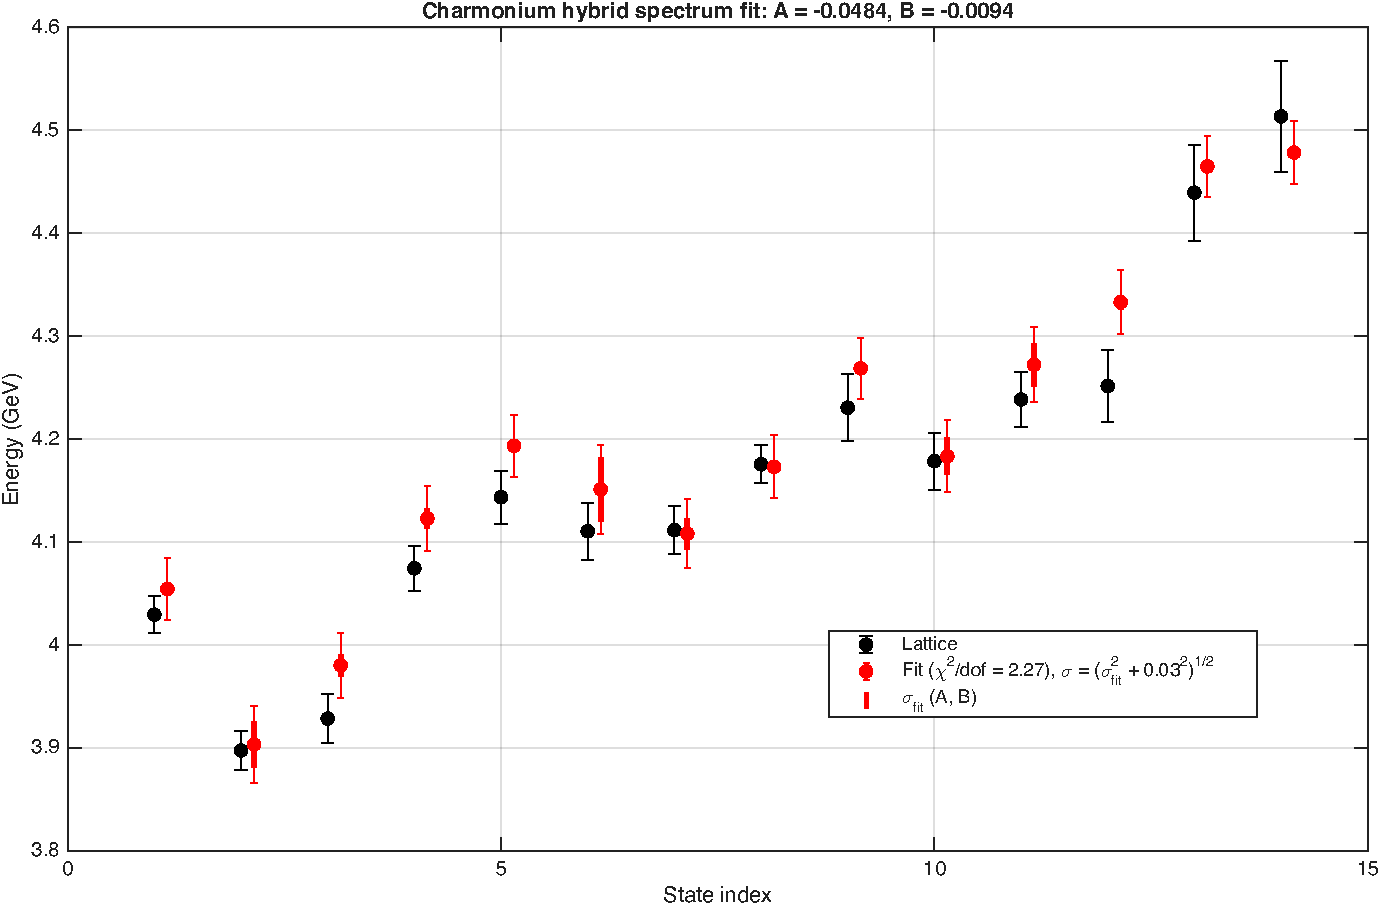
\includegraphics[width=0.49\linewidth]{Fig/fit_nomix.pdf}
    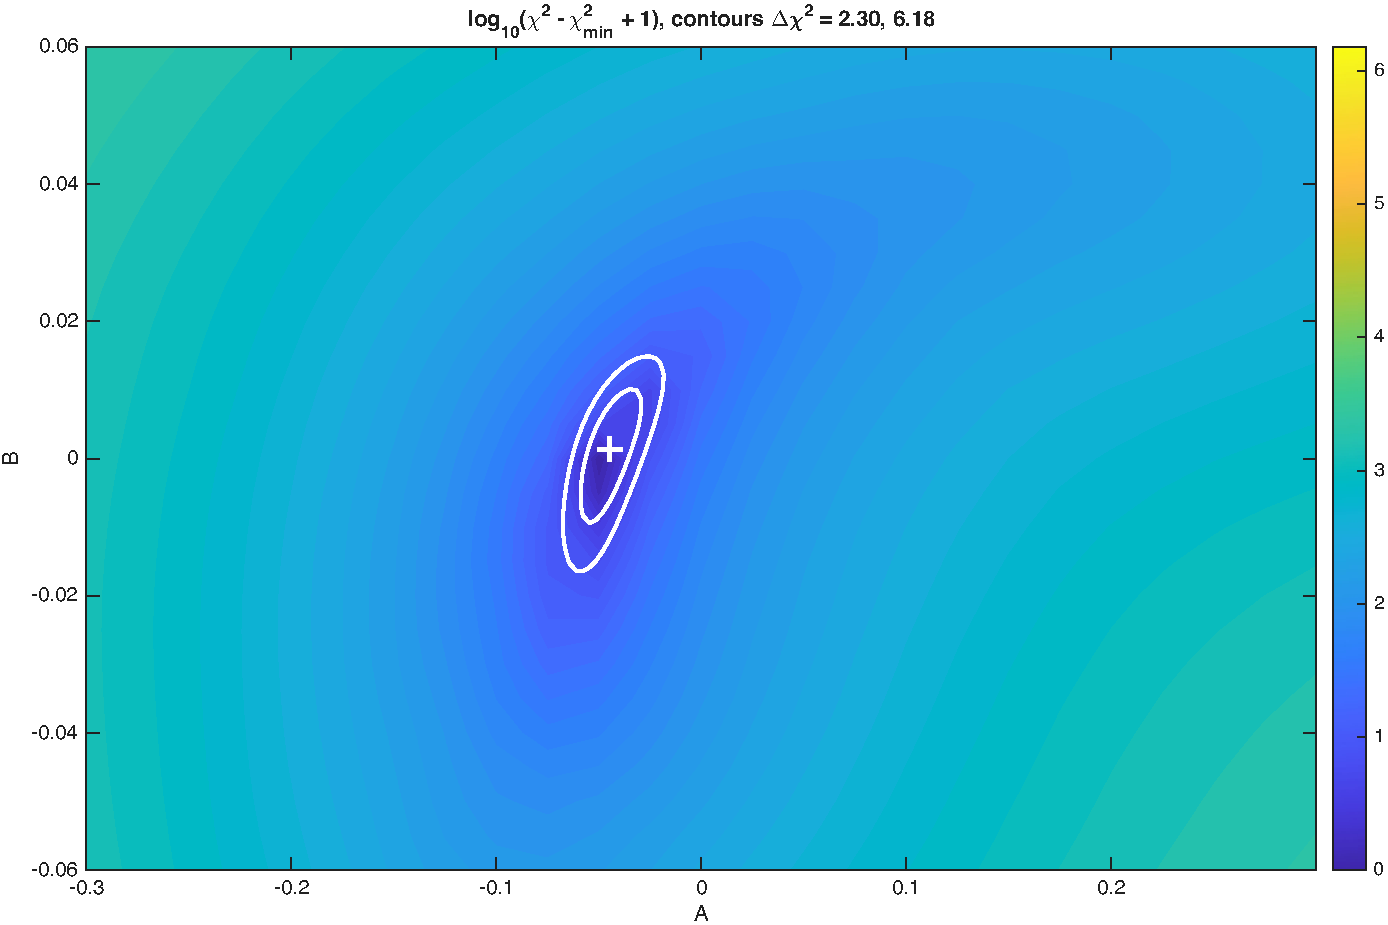
\includegraphics[width=0.49\linewidth]{Fig/chi2_nomix.pdf}
    \caption{\small Best fit without mixing. Left: lattice data (black) and fitted energies (red, shifted to the right) with $\sigma_E$ (thin bar) and $\sigma_{\rm fit}$ (thick bar), in the order of Table~\ref{tab:mass_spectrum}. Right: $\log_{10}(\chi^2-\chi^2_{\rm min}+1)$ in the $(A,B)$ plane with the contours $\Delta\chi^2=2.30$ and $6.18$ (68\% and 95\% for two parameters, unscaled) around the minimum (cross). The tilt of the contours is the correlation $\rho(A,B)$.}
    \label{fig:fit_nomix}
\end{figure}

\begin{figure}[htbp]
    \centering
    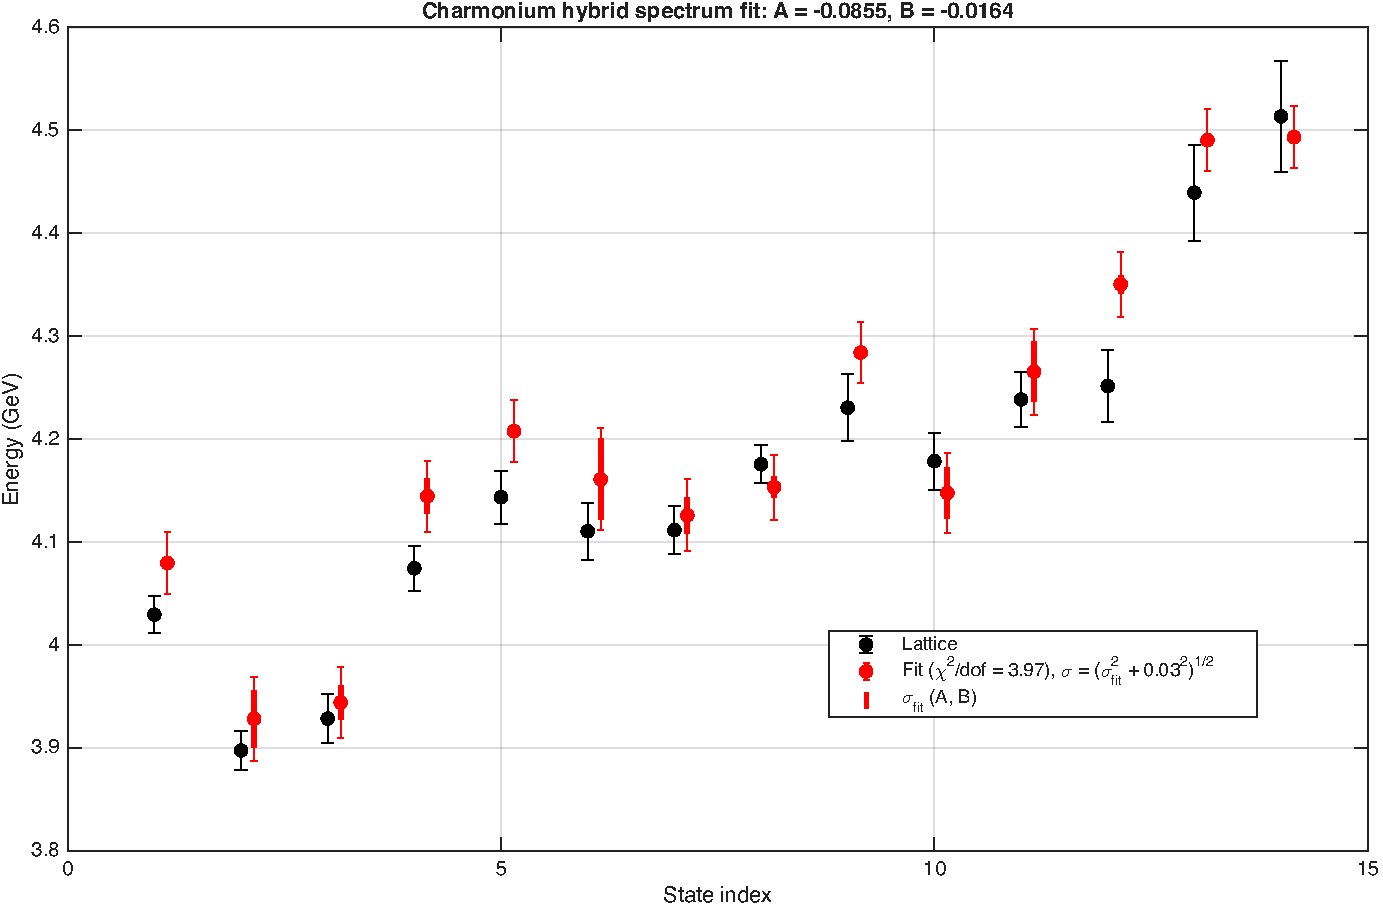
\includegraphics[width=0.49\linewidth]{Fig/fit_mix.pdf}
    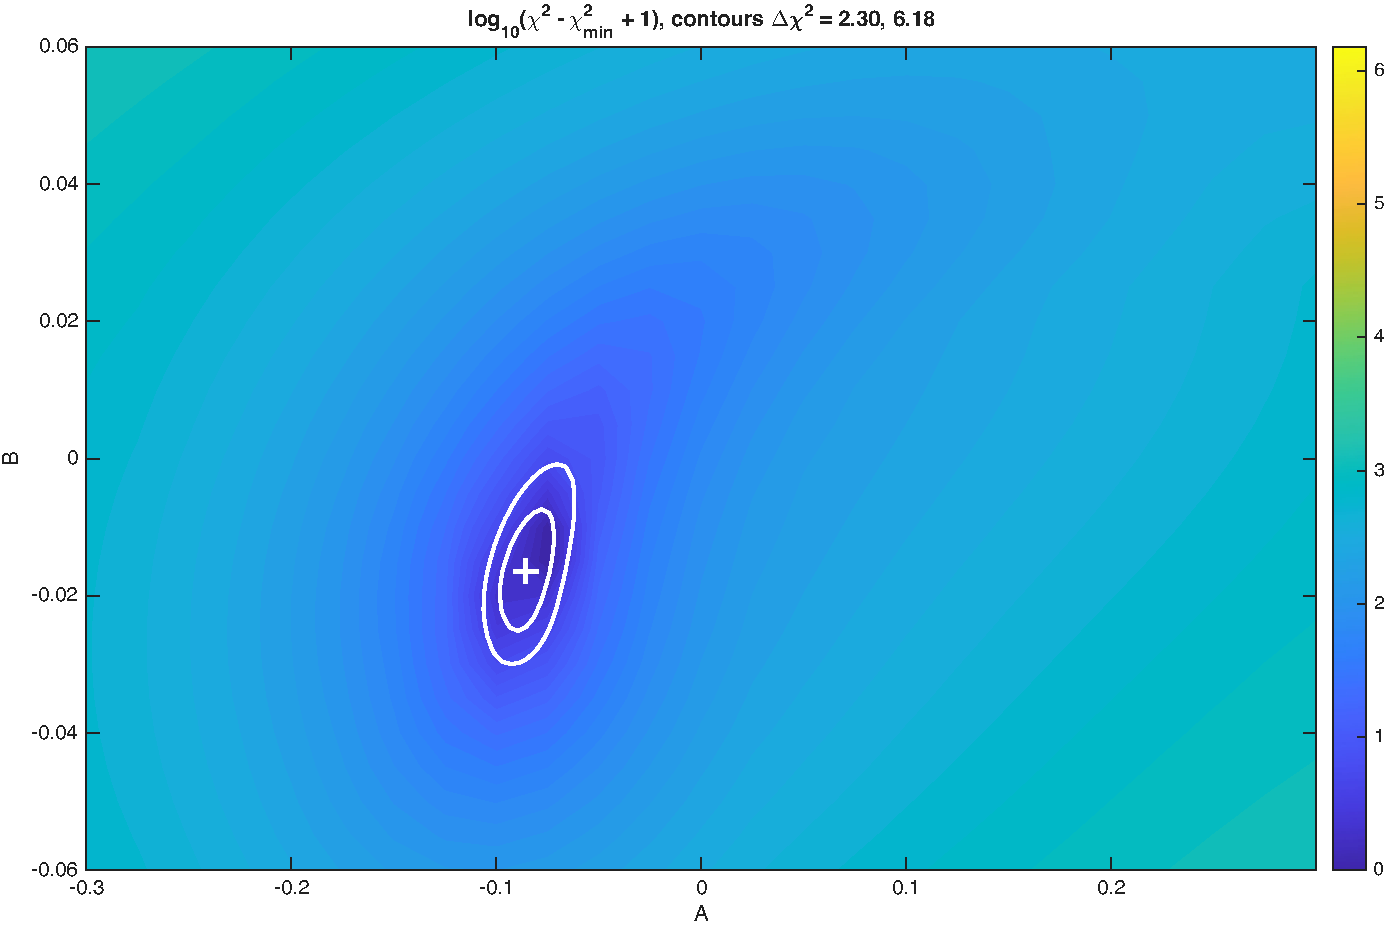
\includegraphics[width=0.49\linewidth]{Fig/chi2_mix.pdf}
    \caption{\small Same as Fig.~\ref{fig:fit_nomix} for the best fit with mixing.}
    \label{fig:fit_mix}
\end{figure}

\printbibliography

\end{document}
